\documentclass[14pt,a4paper,oneside]{extbook}
\usepackage[utf8]{inputenc}
\usepackage[T1]{fontenc}
\usepackage[spanish,es-lcroman]{babel}
\usepackage{libertine}
\usepackage[top=3cm,bottom=3cm,left=3cm,right=3cm,headheight=52pt,headsep=10pt]{geometry}
\usepackage{xcolor}
\usepackage{graphicx}
\usepackage{eso-pic}
\usepackage{fancyhdr}
\usepackage{titlesec}
\usepackage{enumitem}
\usepackage{microtype}
\usepackage{csquotes}
\usepackage{tcolorbox}
\usepackage{hyperref}
\usepackage{bookmark}
\usepackage{parskip}
\usepackage{setspace}
\usepackage{tabularx}   % For flexible, auto-fitting columns
\usepackage{array}      % For advanced column formatting

\setstretch{1.2}
\usepackage{booktabs}
\definecolor{primary}{HTML}{1A365D} % Deep Navy
\definecolor{secondary}{HTML}{2B6CB0} % Slate Blue
\definecolor{accent}{HTML}{C53030} % Warm Red
\hypersetup{
    colorlinks=true,
    linkcolor=primary,
    filecolor=accent,
    urlcolor=secondary,
    citecolor=primary,
    pdftitle={Arquitectura Metodológica LAZY-LOL},
    pdfauthor={Gabriel A. Morales M.}
}
\setlist[itemize]{leftmargin=2.5em, label=\textcolor{secondary}{\textbullet}, noitemsep, topsep=0.5ex}
\newtcolorbox{keyquestion}{
  colback=secondary!5,
  colframe=secondary!30,
  left=1.5em,
  right=1.5em,
  top=1em,
  bottom=1em,
  arc=5pt,
  boxrule=1pt,
  fontupper=\itshape\color{primary},
  halign=center
}
\newtcolorbox{authorobservation}{
  colback=primary!5,
  colframe=primary!30,
  left=1.5em,
  right=1.5em,
  top=1em,
  bottom=1em,
  arc=5pt,
  boxrule=1pt,
  fontupper=\color{primary},
  title=\textbf{Observación del Autor},
  coltitle=primary,
  fonttitle=\sffamily\bfseries,
  attach title to upper=\par\vspace{0.5em}
}
\newenvironment{referenceslist}{
  \begin{list}{}{
    \setlength{\leftmargin}{2.5em}
    \setlength{\itemindent}{-2.5em}
    \setlength{\parsep}{0.6em}
    \setlength{\itemsep}{0pt}
  }
}{
  \end{list}
}
\pagestyle{fancy}
\fancyhf{}
\fancyhead[R]{\sffamily\color{secondary}\leftmark}
\fancyfoot[C]{\sffamily\color{primary}\thepage}
\renewcommand{\headrulewidth}{0.5pt}
\renewcommand{\footrulewidth}{0pt}
\fancypagestyle{plain}{
  \fancyhf{}
  \fancyfoot[C]{\sffamily\color{primary}\thepage}
  \renewcommand{\headrulewidth}{0pt}
}
\titleformat{\chapter}[display]
  {\normalfont\huge\bfseries\color{primary}}
  {\filleft\textsf{\fontsize{50}{50}\selectfont\color{secondary!25}\thechapter}}
  {10pt}
  {\filleft\Huge}
  [\vspace{1ex}\titlerule]
\titleformat{name=\chapter,numberless}[display]
  {\normalfont\huge\bfseries\color{primary}}
  {}
  {0pt}
  {\filleft\Huge}
  [\vspace{1ex}\titlerule]
\titleformat{\section}
  {\normalfont\Large\bfseries\color{primary}}
  {\thesection}{1em}{}
\titleformat{\subsection}
  {\normalfont\large\bfseries\color{secondary}}
  {\thesubsection}{1em}{}
\begin{document}
\begin{titlepage}
\AddToShipoutPictureBG*{%
  \AtPageLowerLeft{%
    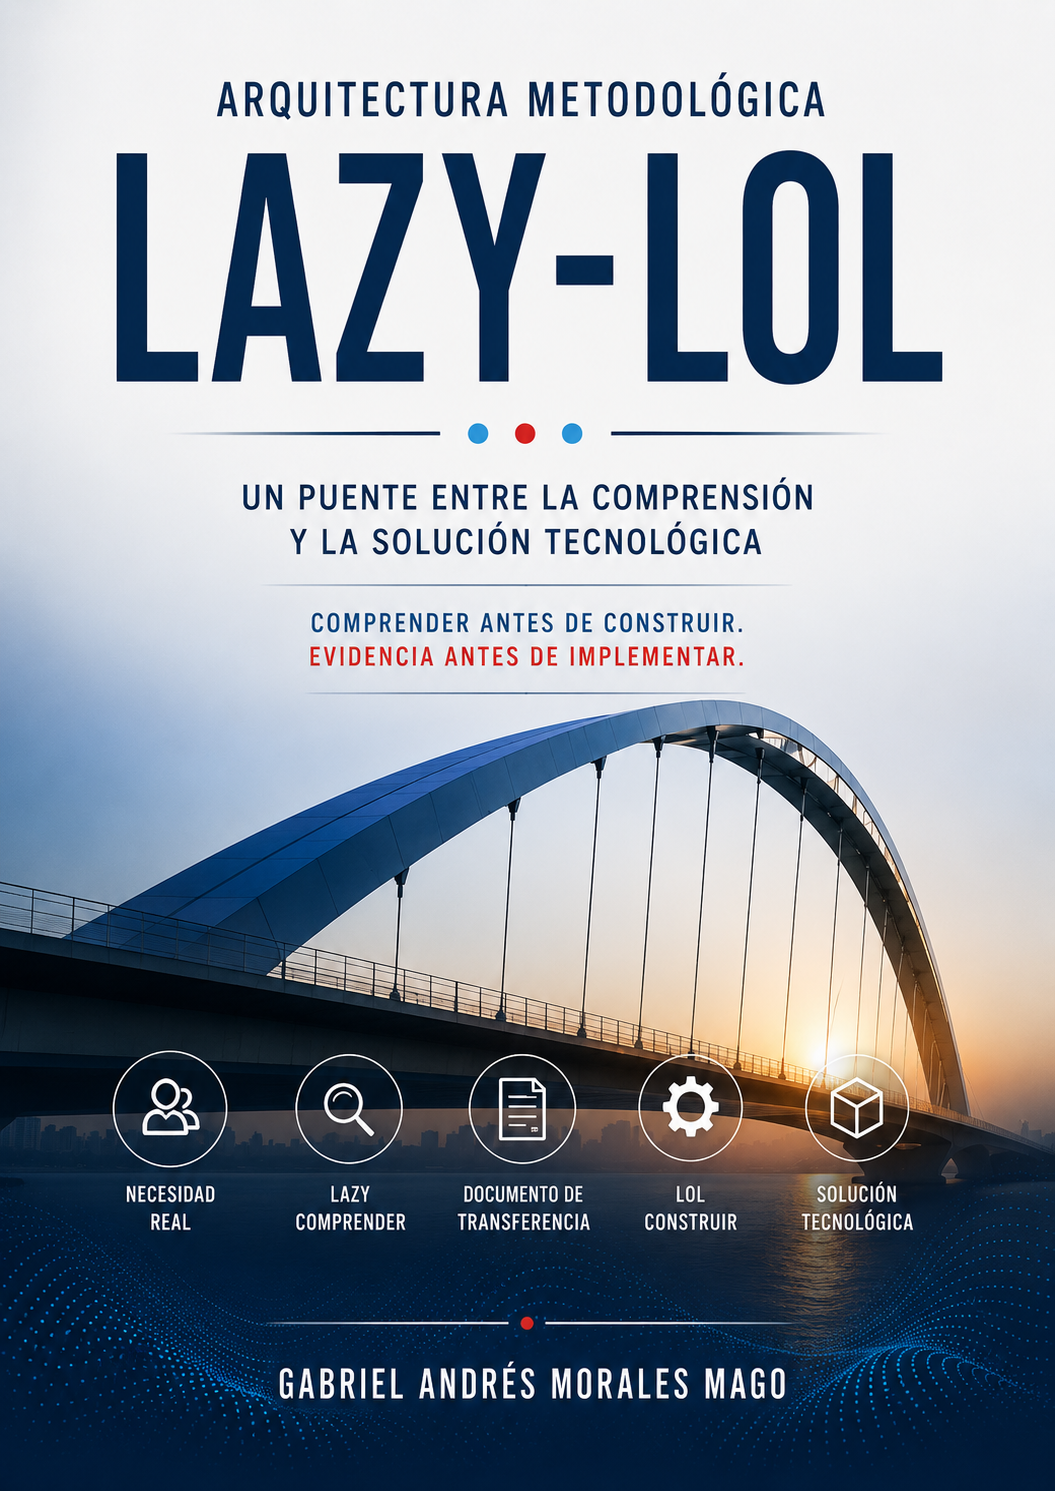
\includegraphics[width=\paperwidth,height=\paperheight]{imagenes/newCover.png}%
  }%
}
\phantom{.}
\newpage
\end{titlepage}
\frontmatter
\tableofcontents
\chapter*{Nota del Autor sobre la Accesibilidad}
\addcontentsline{toc}{chapter}{Nota del Autor sobre la Accesibilidad}
Uno de los principios centrales de este libro es comprender a las personas antes de construir soluciones para ellas. Siguiendo esa misma filosofía, esta edición utiliza un tamaño de fuente mayor al convencional (14pt) y un espaciado interlineal optimizado para favorecer una experiencia de lectura más cómoda y accesible, especialmente para personas con dificultades visuales.
\par\vspace{1em}
Las mejores soluciones tecnológicas no se construyen únicamente para los usuarios promedio; también deben considerar las necesidades de quienes suelen quedar fuera del diseño inicial. Espero que esta pequeña decisión de diseño editorial contribuya a que el conocimiento contenido en estas páginas pueda llegar a más lectores con total comodidad.
\newpage
\mainmatter
\chapter{Introducción}
El desarrollo de software moderno enfrenta un desafío constante: equilibrar las necesidades reales de los usuarios con la implementación técnica de soluciones eficientes, seguras y sostenibles. A lo largo de los años han surgido numerosos marcos de trabajo y metodologías, tales como Agile, Scrum, Kanban y Extreme Programming (XP), los cuales han contribuido significativamente a la organización de equipos y proyectos de software. Sin embargo, muchos de estos enfoques fueron diseñados para entornos donde se asume una participación activa y relativamente equilibrada de todos los integrantes del equipo.

En el contexto académico, especialmente en proyectos socio-tecnológicos desarrollados por estudiantes universitarios, esta premisa no siempre se cumple. Los equipos suelen estar conformados por miembros con distintos niveles de experiencia, disponibilidad, motivación y compromiso. Como consecuencia, la ejecución del proyecto puede depender de uno o pocos integrantes, mientras que otros participan de manera limitada o exclusivamente observacional. Aunque esta situación es frecuente, pocas metodologías la abordan de forma explícita.

Adicionalmente, los proyectos socio-tecnológicos presentan una particularidad que no siempre es considerada por los marcos tradicionales de desarrollo: antes de construir una solución tecnológica, es necesario comprender un problema social. Esto implica realizar actividades de investigación, observación, análisis y validación con comunidades o grupos de interés, generando un conjunto de requisitos que posteriormente servirán como base para el desarrollo del software.

Con el objetivo de abordar ambos desafíos, este trabajo propone una arquitectura metodológica compuesta por dos marcos complementarios: LAZY y LOL.

LAZY (Listen, Analyze, Zoom, Yield) es un marco de investigación socio-tecnológica orientado a identificar, analizar y transformar necesidades sociales en requisitos técnicamente accionables. Su propósito principal es reducir la distancia existente entre el diagnóstico social y la planificación del desarrollo, proporcionando un proceso estructurado para convertir observaciones y hallazgos en objetivos concretos de software.

Por su parte, LOL (Logic, Oversight, Layering) es un marco de desarrollo de software centrado en la definición lógica del sistema, la supervisión continua de la calidad y la seguridad, y la construcción por capas de soluciones tecnológicas. LOL incorpora principios de ingeniería de software, aseguramiento de calidad y pensamiento orientado a la seguridad, promoviendo ciclos iterativos de construcción y validación.

Una característica distintiva de LOL es la incorporación de roles de participación adaptativa. En lugar de asumir que todos los miembros del equipo desempeñarán funciones técnicas equivalentes, el marco reconoce distintos niveles de contribución, permitiendo la existencia de participantes con responsabilidades de observación, validación o representación de usuarios. Esta aproximación busca reflejar de manera más realista la dinámica de numerosos proyectos académicos y multidisciplinarios.

La integración de ambos marcos establece un flujo continuo que inicia con la identificación de una necesidad social mediante LAZY y culmina con la implementación de una solución tecnológica a través de LOL. De esta forma, se propone una visión unificada donde la investigación social y el desarrollo de software dejan de ser procesos independientes para convertirse en componentes de una misma estrategia de resolución de problemas.

Finalmente, este documento presenta los fundamentos conceptuales de ambos marcos, sus roles, ciclos y mecanismos de integración, así como un caso de estudio basado en el desarrollo de una aplicación de gestión de tareas. El objetivo es evaluar la viabilidad de esta propuesta como una alternativa adaptable para proyectos socio-tecnológicos en contextos académicos y profesionales.

Y sí, aunque los nombres LAZY y LOL puedan parecer poco convencionales en un primer momento, la ingeniería de software ha demostrado repetidamente que las buenas ideas no dependen de nombres serios, sino de resultados serios.


\chapter*{Manifiesto LOL-LAZY}
\addcontentsline{toc}{chapter}{Manifiesto LOL-LAZY}

\begin{enumerate}
\item Las necesidades reales por encima de las suposiciones.
\item La evidencia por encima de la intuición no validada.
\item La simplicidad por encima de la complejidad preventiva.
\item La adaptación por encima de la rigidez metodológica.
\item Las personas por encima de los artefactos.
\item La comprensión antes de la implementación.
\item La trazabilidad entre problema y solución.
\item El impacto social por encima del volumen de código.
\end{enumerate}

\chapter{El Puente Perdido}

\begin{keyquestion}
Problema Real $\rightarrow$ LAZY $\rightarrow$ Documento de Transferencia $\rightarrow$ LOL $\rightarrow$ Solución Tecnológica
\end{keyquestion}

La tesis central de este libro es que el software no comienza con código.
Comienza con una necesidad humana. LAZY proporciona una estructura para comprender
esa necesidad. LOL proporciona una estructura para transformar esa comprensión en una
solución tecnológica trazable.

\begin{authorobservation}
La idea más importante de este libro no es LAZY ni LOL por separado, sino el puente que
existe entre ambos. Una solución tecnológica pierde valor cuando se desconecta del problema
que le dio origen.
\end{authorobservation}



El desarrollo de software moderno enfrenta un desafío constante: equilibrar las necesidades reales de los usuarios con la implementación técnica de soluciones eficientes, seguras y sostenibles. A lo largo de los años han surgido numerosos marcos de trabajo y metodologías, tales como Agile, Scrum, Kanban y Extreme Programming (XP), los cuales han contribuido significativamente a la organización de equipos y proyectos de software. Sin embargo, muchos de estos enfoques fueron diseñados para entornos donde se asume una participación activa y relativamente equilibrada de todos los integrantes del equipo.

En el contexto académico, especialmente en proyectos socio-tecnológicos desarrollados por estudiantes universitarios, esta premisa no siempre se cumple. Los equipos suelen estar conformados por miembros con distintos niveles de experiencia, disponibilidad, motivación y compromiso. Como consecuencia, la ejecución del proyecto puede depender de uno o pocos integrantes, mientras que otros participan de manera limitada o exclusivamente observacional. Aunque esta situación es frecuente, pocas metodologías la abordan de forma explícita.

Adicionalmente, los proyectos socio-tecnológicos presentan una particularidad que no siempre es considerada por los marcos tradicionales de desarrollo: antes de construir una solución tecnológica, es necesario comprender un problema social. Esto implica realizar actividades de investigación, observación, análisis y validación con comunidades o grupos de interés, generando un conjunto de requisitos que posteriormente servirán como base para el desarrollo del software.

Con el objetivo de abordar ambos desafíos, este trabajo propone una arquitectura metodológica compuesta por dos marcos complementarios: LAZY y LOL.

LAZY (Listen, Analyze, Zoom, Yield) es un marco de investigación socio-tecnológica orientado a identificar, analizar y transformar necesidades sociales en requisitos técnicamente accionables. Su propósito principal es reducir la distancia existente entre el diagnóstico social y la planificación del desarrollo, proporcionando un proceso estructurado para convertir observaciones y hallazgos en objetivos concretos de software.

Por su parte, LOL (Logic, Oversight, Layering) es un marco de desarrollo de software centrado en la definición lógica del sistema, la supervisión continua de la calidad y la seguridad, y la construcción por capas de soluciones tecnológicas. LOL incorpora principios de ingeniería de software, aseguramiento de calidad y pensamiento orientado a la seguridad, promoviendo ciclos iterativos de construcción y validación.

Una característica distintiva de LOL es la incorporación de roles de participación adaptativa. En lugar de asumir que todos los miembros del equipo desempeñarán funciones técnicas equivalentes, el marco reconoce distintos niveles de contribución, permitiendo la existencia de participantes con responsabilidades de observación, validación o representación de usuarios. Esta aproximación busca reflejar de manera más realista la dinámica de numerosos proyectos académicos y multidisciplinarios.

La integración de ambos marcos establece un flujo continuo que inicia con la identificación de una necesidad social mediante LAZY y culmina con la implementación de una solución tecnológica a través de LOL. De esta forma, se propone una visión unificada donde la investigación social y el desarrollo de software dejan de ser procesos independientes para convertirse en componentes de una misma estrategia de resolución de problemas.

Finalmente, este documento presenta los fundamentos conceptuales de ambos marcos, sus roles, ciclos y mecanismos de integración, así como un caso de estudio basado en el desarrollo de una aplicación de gestión de tareas. El objetivo es evaluar la viabilidad de esta propuesta como una alternativa adaptable para proyectos socio-tecnológicos en contextos académicos y profesionales.

Y sí, aunque los nombres LAZY y LOL puedan parecer poco convencionales en un primer momento, la ingeniería de software ha demostrado repetidamente que las buenas ideas no dependen de nombres serios, sino de resultados serios.



\chapter{Planteamiento del Problema}

El desarrollo de software y la investigación socio-tecnológica son disciplinas que tradicionalmente han evolucionado de manera paralela. Mientras que los procesos de investigación buscan comprender necesidades humanas, problemáticas sociales y contextos organizacionales, los procesos de desarrollo se enfocan en la construcción de soluciones tecnológicas capaces de responder a dichos desafíos. Sin embargo, en numerosos entornos académicos y profesionales, la transición entre ambas etapas carece de una estructura clara y formalizada.

En los proyectos socio-tecnológicos es común encontrar una desconexión entre el diagnóstico social y la implementación técnica. Los resultados obtenidos durante entrevistas, encuestas, observaciones o análisis comunitarios suelen transformarse en extensos documentos que posteriormente deben ser interpretados por los equipos de desarrollo. Este proceso puede provocar pérdida de información, ambigüedades en los requisitos y dificultades para garantizar que la solución final responda efectivamente a las necesidades identificadas.

Por otra parte, muchos marcos de desarrollo de software contemporáneos fueron diseñados bajo la premisa de equipos altamente colaborativos, con niveles de participación relativamente homogéneos entre sus integrantes. En la práctica, especialmente dentro de contextos académicos, esta situación no siempre ocurre. Los equipos suelen estar conformados por personas con distintos niveles de experiencia, disponibilidad, interés o conocimientos técnicos. Como consecuencia, la distribución real del trabajo puede diferir significativamente de la distribución teórica planteada por las metodologías tradicionales.

Esta diferencia entre los modelos ideales y las condiciones reales genera diversos problemas. Entre ellos destacan la sobrecarga de ciertos integrantes del equipo, la dificultad para asignar responsabilidades adecuadas a participantes con perfiles no técnicos, la falta de mecanismos formales para integrar contribuciones observacionales o consultivas y la ausencia de procesos que permitan mantener la continuidad del proyecto cuando la participación del equipo es desigual.

Adicionalmente, el creciente uso de herramientas basadas en inteligencia artificial, automatización y análisis asistido por software plantea nuevas oportunidades que aún no son abordadas de manera explícita por muchos marcos tradicionales. La capacidad de utilizar sistemas inteligentes para apoyar procesos de investigación, validación, supervisión y desarrollo abre la posibilidad de replantear la forma en que se estructuran los proyectos socio-tecnológicos.

Ante esta situación surge la necesidad de una propuesta que permita integrar de forma coherente la investigación social y el desarrollo de software, al mismo tiempo que reconoce la diversidad de roles y niveles de participación presentes en equipos reales.

Por ello, este trabajo propone una arquitectura compuesta por dos marcos complementarios: LAZY, orientado a la investigación y validación socio-tecnológica, y LOL, orientado al desarrollo de software, supervisión y construcción iterativa de soluciones. Ambos marcos buscan establecer un flujo continuo desde la identificación de un problema social hasta la entrega de un producto funcional, reduciendo la brecha existente entre la investigación y la implementación tecnológica.

La pregunta central que guía esta propuesta es la siguiente:

\begin{keyquestion}
¿Es posible diseñar una arquitectura metodológica que permita transformar necesidades sociales en soluciones tecnológicas mediante un proceso estructurado, adaptable y compatible con equipos de participación variable, manteniendo la calidad técnica y la relevancia social del resultado final?
\end{keyquestion}

\begin{authorobservation}
Durante mis primeros proyectos universitarios asumía que el principal desafío sería programar. Con el tiempo descubrí que el problema más difícil era entender qué debía construirse y por qué. En varias ocasiones observé equipos capaces de producir grandes cantidades de código para resolver problemas que nunca habían sido definidos correctamente.

Esta experiencia me llevó a valorar la investigación previa como una actividad de ingeniería y no simplemente como un requisito académico.
\end{authorobservation}


\chapter{Marco Teórico y Trabajos Relacionados}

\section{Introducción}

El desarrollo de software ha evolucionado significativamente durante las últimas décadas. A medida que los sistemas se han vuelto más complejos, las organizaciones y los equipos de trabajo han requerido mecanismos que permitan coordinar esfuerzos, administrar recursos y garantizar la calidad de los productos desarrollados.

Como respuesta a esta necesidad han surgido numerosas metodologías y marcos de trabajo que buscan estructurar el proceso de desarrollo. Entre los más influyentes se encuentran Agile, Scrum, Kanban y Extreme Programming (XP), los cuales han servido como referencia para miles de equipos alrededor del mundo.

Paralelamente, en el ámbito de la investigación aplicada han surgido enfoques como Design Science Research y Action Research, orientados a la resolución sistemática de problemas mediante la creación de artefactos o la intervención directa sobre contextos reales.

El análisis de estas propuestas permite identificar fortalezas importantes, pero también ciertas limitaciones cuando se aplican a proyectos socio-tecnológicos desarrollados en contextos académicos, especialmente aquellos caracterizados por equipos pequeños, recursos limitados y niveles variables de participación entre sus integrantes.

\par\vspace{1.5em}\noindent\hfill\rule{0.25\textwidth}{0.6pt}\hfill\par\vspace{1.5em}

\section{Agile}

Agile no constituye una metodología específica, sino una filosofía de desarrollo basada en principios de adaptación, colaboración y entrega continua de valor.

El Manifiesto Ágil propone priorizar a las personas sobre los procesos rígidos, el software funcional sobre la documentación excesiva, la colaboración con el cliente sobre la negociación contractual y la capacidad de respuesta al cambio sobre el seguimiento estricto de planes previamente definidos.

La principal contribución de Agile fue cuestionar los modelos secuenciales tradicionales y promover una visión iterativa del desarrollo de software.

Sin embargo, Agile asume una interacción frecuente entre los miembros del equipo y una participación activa de todos los involucrados. En contextos donde la distribución real del trabajo es desigual, la aplicación práctica de algunos de sus principios puede resultar más compleja de lo esperado.

\par\vspace{1.5em}\noindent\hfill\rule{0.25\textwidth}{0.6pt}\hfill\par\vspace{1.5em}

\section{Scrum}

Scrum es uno de los marcos ágiles más difundidos en la industria del software.

Su estructura se basa en ciclos cortos denominados Sprints, dentro de los cuales el equipo desarrolla incrementos funcionales del producto. Scrum define roles específicos como Product Owner, Scrum Master y Development Team, además de ceremonias periódicas para la planificación, seguimiento y revisión del trabajo realizado.

Entre sus ventajas destacan la transparencia, la capacidad de adaptación y la mejora continua.

No obstante, Scrum fue concebido para equipos altamente colaborativos y con niveles relativamente homogéneos de participación. La efectividad de muchas de sus prácticas depende de la existencia de comunicación constante, responsabilidad compartida y compromiso activo de todos los integrantes.

En proyectos académicos, estas condiciones no siempre se presentan de forma consistente.

\par\vspace{1.5em}\noindent\hfill\rule{0.25\textwidth}{0.6pt}\hfill\par\vspace{1.5em}

\section{Kanban}

Kanban es un marco de gestión visual orientado a optimizar el flujo de trabajo.

Su principal característica consiste en representar tareas mediante tableros visuales que permiten observar el estado actual de cada actividad. Este enfoque facilita la identificación de cuellos de botella y promueve una mejora continua basada en datos observables.

Una de las fortalezas de Kanban es su simplicidad y flexibilidad, ya que puede integrarse fácilmente con otros enfoques de desarrollo.

Sin embargo, Kanban se concentra principalmente en la gestión del flujo de trabajo y no proporciona mecanismos específicos para abordar aspectos relacionados con la investigación social, la validación de necesidades comunitarias o la adaptación a distintos niveles de participación dentro de los equipos.

\par\vspace{1.5em}\noindent\hfill\rule{0.25\textwidth}{0.6pt}\hfill\par\vspace{1.5em}

\section{Extreme Programming (XP)}

Extreme Programming (XP), propuesta por Kent Beck, constituye una de las metodologías ágiles más influyentes dentro de la ingeniería de software.

XP promueve prácticas orientadas a maximizar la calidad del código y la capacidad de adaptación frente a cambios en los requisitos. Entre sus prácticas más conocidas se encuentran la programación en parejas, la integración continua, las pruebas automatizadas y la refactorización constante.

Uno de los principios fundamentales de XP es que la simplicidad constituye una ventaja estratégica. En lugar de intentar predecir todos los escenarios futuros, XP propone desarrollar únicamente aquello que resulta necesario en el momento actual, permitiendo que el sistema evolucione gradualmente.

Esta filosofía resulta especialmente atractiva para proyectos académicos y equipos pequeños, ya que favorece la construcción incremental de soluciones funcionales.

Sin embargo, varias de las prácticas centrales de XP fueron diseñadas bajo la premisa de una colaboración intensa entre desarrolladores. Actividades como la programación en parejas o la propiedad colectiva del código pueden resultar difíciles de implementar cuando la participación efectiva del equipo es desigual.

A pesar de ello, XP aporta una visión valiosa sobre la importancia de la simplicidad, la retroalimentación constante y la mejora continua, principios que influyen directamente en el diseño del marco LOL.

\par\vspace{1.5em}\noindent\hfill\rule{0.25\textwidth}{0.6pt}\hfill\par\vspace{1.5em}

\section{Design Science Research}

Design Science Research (DSR) es un enfoque de investigación orientado a la creación de artefactos capaces de resolver problemas identificados en contextos reales.

Dentro de este paradigma, un artefacto puede tomar diversas formas, incluyendo modelos, métodos, procesos, algoritmos o sistemas de software.

La principal contribución de DSR consiste en considerar la construcción de soluciones como una actividad científica válida, permitiendo que el conocimiento se genere a través del diseño, implementación y evaluación de dichas soluciones.

Este enfoque resulta particularmente relevante para proyectos de ingeniería de software, ya que legitima la creación de nuevos marcos, herramientas y procesos como contribuciones académicas.

\par\vspace{1.5em}\noindent\hfill\rule{0.25\textwidth}{0.6pt}\hfill\par\vspace{1.5em}

\section{Action Research}

Action Research es una metodología de investigación basada en la intervención directa sobre una realidad específica con el objetivo de comprenderla y mejorarla simultáneamente.

Su estructura suele desarrollarse mediante ciclos de observación, análisis, acción y reflexión.

A diferencia de enfoques puramente descriptivos, Action Research busca generar cambios concretos dentro del contexto estudiado mientras produce conocimiento sobre dicho proceso.

Esta metodología resulta especialmente compatible con proyectos socio-tecnológicos, debido a que permite trabajar de forma cercana con comunidades, organizaciones o grupos de usuarios reales.

Muchos de los principios presentes en LAZY encuentran inspiración en esta perspectiva de investigación aplicada.

\par\vspace{1.5em}\noindent\hfill\rule{0.25\textwidth}{0.6pt}\hfill\par\vspace{1.5em}

\section{Limitaciones Identificadas}

El análisis de los enfoques estudiados permite identificar una serie de limitaciones comunes cuando son aplicados a proyectos socio-tecnológicos desarrollados en entornos académicos.

En primer lugar, existe una separación frecuente entre la fase de investigación social y la fase de desarrollo técnico, generando dificultades para transformar hallazgos sociales en requisitos de software claramente definidos.

En segundo lugar, la mayoría de los marcos analizados asumen equipos altamente colaborativos y niveles relativamente homogéneos de participación. Esta situación no siempre refleja la realidad de numerosos proyectos académicos, donde los integrantes pueden contribuir de formas distintas y en diferentes niveles.

Finalmente, aunque estos enfoques proporcionan mecanismos sólidos para gestionar el desarrollo de software o la investigación aplicada de forma independiente, pocos ofrecen una integración explícita entre ambas dimensiones.

Estas limitaciones constituyen la motivación principal para la propuesta de los marcos LAZY y LOL, los cuales buscan establecer una conexión estructurada entre la investigación socio-tecnológica y el desarrollo de software, incorporando además un modelo de participación adaptable a las condiciones reales de trabajo observadas en numerosos proyectos académicos.



\chapter{El Proyecto Socio-Integrador/Tecnológico como Contexto de Investigación}
\section{Introducción: Un Formato que No Es una Tesis}
\begin{itemize}
\item Quien no conoce el sistema universitario venezolano podría asumir que el Proyecto Socio-Integrador/Tecnológico (PSI/T) es simplemente el equivalente local de una tesis de grado. Sería un error comprensible, pero tiene consecuencias metodológicas importantes. El PSI/T no es una tesis. No llega hasta proponer una solución y detenerse. No vive en el papel. Requiere un producto tangible, un beneficiario real y una comunidad que lo use. Entender esta diferencia es indispensable para comprender por qué los frameworks LOL y LAZY surgen de ese contexto específico y no de otro.
\item Este capítulo explica qué es el PSI/T, cómo se organiza dentro del sistema de Programas Nacionales de Formación (PNF), cuáles son sus reglas reales y, sobre todo, por qué las metodologías convencionales que se enseñan en los PNF ---XP, historias de usuario, UML--- asumen condiciones que ese contexto raramente cumple.
\end{itemize}
\section{Qué es el PSI/T: Definición Oficial y sus Implicaciones}
\begin{itemize}
\item El Reglamento para la Administración del Proyecto Socio Integrador/Tecnológico de la Universidad Politécnica Territorial del Estado Trujillo \enquote{Mario Briceño Iragorry} (UPTT-MBI), aprobado en sesión extraordinaria del Consejo Directivo Provisional N° CDP EXT 062-A-17 el 15 de mayo de 2017, define el PSI/T en su Artículo 2 de la siguiente manera:
\item \enquote{El Proyecto Socio Integrador/Tecnológico (PSI/T) es una unidad curricular de integración de saberes y contraste entre teoría y práctica, vinculada a la producción de bienes o prestación de servicios, asociados al desarrollo de capacidades, generación de conocimientos, investigación, innovación, creación artística, desarrollo tecnológico y fortalecimiento del poder popular. Constituye el eje transversal de la formación académica, desarrollado en los respectivos trayectos que conforman el Programa Nacional de Formación.} (Artículo 2, Reglamento PSIT, 2017)
\item Hay tres elementos en esa definición que merecen análisis separado. Primero, es una unidad curricular de integración: no es optativa, no es un proyecto libre, es el eje que cruza toda la formación. Segundo, está vinculada a producción de bienes o servicios: no a propuestas ni a modelos teóricos, sino a resultados concretos que deben existir fuera del papel. Tercero, incluye explícitamente el fortalecimiento del poder popular entre sus propósitos, lo que lo sitúa en una tradición de educación comunitaria con raíces políticas e históricas definidas.
\item El Artículo 3 refuerza el carácter obligatorio del PSI/T: es requisito para obtener las certificaciones y titulaciones correspondientes a cada trayecto. El Artículo 4 lo describe como eje que integra práctica profesional, servicio comunitario y vinculación social. Y el Artículo 10 añade que debe ser desarrollado \enquote{en conjunto con la comunidad, desde lo simple a lo más complejo}. En otras palabras: no hay PSI/T válido sin una comunidad real involucrada.
\end{itemize}
\section{La Estructura por Trayectos y las Líneas de Investigación}
\begin{itemize}
\item El sistema de PNF no organiza sus estudios en años académicos tradicionales sino en trayectos, numerados en cifras romanas. Cada trayecto tiene asociada una línea de investigación que define el tipo de producto tecnológico esperado del PSI/T. Esta estructura es crucial para entender el nivel de complejidad creciente que el estudiante debe manejar.
\item En el Programa Nacional de Formación en Informática ---el contexto del caso de estudio desarrollado en capítulos anteriores--- las líneas de investigación por trayecto se distribuyen aproximadamente así:
\item Trayecto I:  Reparación y mantenimiento de equipos. El estudiante aún no diseña sistemas completos; aprende a intervenir tecnología existente en contextos comunitarios.
\item Trayecto II:  Desarrollo de páginas web. Se introduce el diseño de soluciones digitales básicas con impacto visual y comunicacional para la comunidad.
\item Trayecto III:  Sistema de información. El estudiante debe diseñar, implementar y desplegar un sistema funcional que resuelva un problema de gestión de datos en la comunidad.
\item Trayecto IV:  Aplicación Android. El producto debe ser una aplicación móvil funcional con despliegue real.
\item El Reglamento precisa en su Artículo 7h que \enquote{cada Proyecto Socio Integrador/Tecnológico debe ser desarrollado en función de las líneas de Investigación de cada programa nacional de formación y aquellas que surjan de la interacción con la realidad de las comunidades}. La formulación es relevante: las líneas de investigación no son abstractas sino que se ajustan a lo que la comunidad efectivamente necesita. El estudiante llega con una línea de referencia pero debe negociarla con la realidad del campo.
\item El reglamento también permite que el estudiante proponga una alternativa tecnológica diferente, siempre que esté al menos al mismo nivel de complejidad que la línea oficial de su trayecto. Esto le otorga al PSI/T una flexibilidad real que raramente se menciona en los manuales metodológicos, pero que en la práctica significa que el investigador-desarrollador tiene agencia sobre la solución que elige construir.
\end{itemize}
\section{Los Actores del PSI/T: Un Ecosistema de Roles}
\begin{itemize}
\item Una de las características más distintivas del PSI/T frente a otros formatos de trabajo académico es la multiplicidad de actores que deben estar presentes y que tienen roles formales en el proceso. El Artículo 15 del Reglamento establece que en el desarrollo del PSI/T están involucrados:
\item el Comité Técnico de Investigación del PNF, los estudiantes, el Representante del Consejo Comunal u organización comunitaria en el área del proyecto, el Representante Institucional u organizacional del área, y el Docente Asesor Responsable.
\item Cada uno de esos actores tiene atribuciones precisas definidas en los Artículos 16 al 27. El Docente Asesor, por ejemplo, debe acompañar al estudiante tanto en el aula como en la comunidad (Artículo 23b), verificar los avances según la Planilla de Control de Asesoría FPS-02, y verificar la estructura del proyecto final. El Representante Comunitario debe apoyar al estudiante, establecer el plan de trabajo conjunto, e informar por escrito el estatus del proyecto cuando sea requerido (Artículo 27).
\item Lo que este mapa de actores revela, desde una perspectiva metodológica, es que el PSI/T no tiene un único \enquote{cliente} en el sentido en que lo define XP. Tiene al menos cuatro actores con intereses distintos: la comunidad (que quiere que el problema se resuelva), el docente asesor (que quiere que el proceso cumpla con el reglamento), el representante institucional (que actúa como enlace formal), y el estudiante (que debe integrar los intereses de todos mientras construye algo que funcione). Ningún framework diseñado para entornos corporativos fue pensado para gestionar esa complejidad relacional.
\end{itemize}
\section{La Evaluación: Quién Califica y Qué Se Califica}
\begin{itemize}
    \item \textbf{Sistema de evaluación no convencional (Art. 51):} 
    Se aparta de los modelos académicos convencionales. Es sumativa y formativa (escala 1 al 20) e incluye co-evaluación, autoevaluación y hetero-evaluación. 
    \begin{itemize}
        \item \textit{Distribución:} 40\% presentación oral, 60\% avances del proyecto.
    \end{itemize}

    \item \textbf{Comité Evaluador (Art. 48):} 
    Conformado por el estudiante, el Representante del Consejo Comunal, el Representante Institucional y el Docente Asesor.
    \begin{itemize}
        \item \textit{1er trimestre:} La evaluación recae casi completamente en el docente asesor (90\%).
        \item \textit{2do trimestre en adelante:} La comunidad y el representante institucional participan activamente en la calificación.
    \end{itemize}

    \item \textbf{Consecuencia metodológica:} 
    El estudiante es evaluado por actores con criterios de éxito distintos:
    \begin{itemize}
        \item \textbf{Docente:} Cumplimiento del reglamento.
        \item \textbf{Comunidad:} Utilidad del producto.
        \item \textbf{Representante institucional:} Pertinencia.
        \item \textbf{Estudiante:} Autoevaluación.
    \end{itemize}
    \textit{Conclusión:} La metodología debe generar evidencias legibles para \textbf{todos} estos evaluadores simultáneamente, no solo para un cliente técnico.
\end{itemize}
\section{La Estructura del Informe: Lo que el Reglamento Exige}
\begin{itemize}
\item El Anexo 1 del Reglamento establece la estructura formal que debe tener el informe final del PSI/T. Conocerla es importante porque determina cómo debe organizarse y documentarse el proceso de investigación-desarrollo, independientemente de la metodología que el estudiante utilice internamente. La estructura es la siguiente:
\item Parte I --- Descripción del Proyecto
\item Incluye el diagnóstico situacional, la identificación y jerarquización de necesidades, las alternativas de solución, los propósitos y objetivos, el diseño metodológico del plan de acción, la justificación (teórica, técnica, legal, comunitaria) y los beneficiarios directos e indirectos.
\item Parte II --- Marco Referencial
\item Contiene los antecedentes (entre 3 y 5 estudios relacionados, con no más de 5 años de antigüedad) y las bases teóricas o conceptuales (sustentadas en 2 o 3 autores con vigencia de hasta 10 años).
\item Parte III --- Marco Metodológico
\item Define la modalidad metodológica, el tipo de investigación, las técnicas e instrumentos de recolección de información, y las técnicas de procesamiento y análisis de datos.
\item Parte IV --- Producto Final
\item Comprende el desarrollo de los planes de acción, la propuesta en sí misma, los costos y plan de financiamiento, los medios de obtención de recursos económicos, y la evaluación y seguimiento del proyecto.
\item Partes V y VI --- Conclusiones, Recomendaciones y Referencias
\item Cierre del informe con síntesis de resultados, sugerencias derivadas de la experiencia y lista completa de fuentes citadas.
\item Esta estructura revela algo importante: el PSI/T exige documentar el proceso investigativo (Parte III) y el producto tecnológico (Parte IV) en el mismo informe. No son documentos separados. El investigador y el desarrollador son la misma persona, y el informe debe dar cuenta de ambos roles con igual rigor. Esa dualidad es precisamente lo que hace que los frameworks LOL y LAZY sean pertinentes: fueron construidos desde esa experiencia integrada, no desde la separación entre investigación y desarrollo que caracteriza a las disciplinas más maduras.
\end{itemize}
\section{La Tensión Real: Investigar y Desarrollar al Mismo Tiempo}
\begin{itemize}
\item Aquí reside el argumento central de este capítulo. El PSI/T coloca al estudiante en una posición que ningún manual metodológico de ingeniería de software describe adecuadamente: debe ser investigador de campo, desarrollador de software, gestor comunitario y documentador académico, todo al mismo tiempo, con los mismos recursos y en el mismo período de tiempo.
\item Las metodologías ágiles como XP asumen la existencia de un equipo con roles diferenciados: hay un product owner que escribe las historias de usuario, hay desarrolladores que las implementan, hay un coach que facilita el proceso. En el PSI/T de Trayecto III o IV, puede haber un único estudiante que hace todo. O dos. El Artículo 13 del Reglamento establece que el PSI/T debe ser realizado por un mínimo de dos (2) y máximo de tres (3) estudiantes, con posibilidad de llegar a cinco (5) en proyectos de alta complejidad. No hay un equipo de ocho personas. No hay sprints de dos semanas con retrospectivas facilitadas por un Scrum Master certificado.
\item Las historias de usuario, en particular, presentan un problema de fondo que va más allá de la cantidad de personas disponibles. Funcionan bajo un supuesto implícito que nadie menciona: requieren un cliente disponible, articulado y con tiempo para co-construir las tarjetas en el formato estándar (\enquote{Como [rol] quiero [acción] para [beneficio]}). En el contexto del PSI/T, el \enquote{cliente} es frecuentemente una vocera comunitaria, un presidente de consejo comunal o un coordinador de organización social. Estas personas tienen disposición para colaborar, pero no están familiarizadas con el lenguaje de las historias de usuario, no tienen tiempo para sesiones de refinement de backlog y no van a sentarse a escribir criterios de aceptación.
\item Lo que el investigador-desarrollador obtiene en campo es una entrevista grabada en audio, quizás una observación directa de los procesos problemáticos, y la confianza de que quien recibe la tecnología sabe que el estudiante entendió el problema. A partir de esa materia prima, el investigador debe hacer una traducción: convertir frustraciones expresadas en lenguaje coloquial en requerimientos funcionales y no funcionales documentables. Eso no es XP. Es análisis cualitativo con finalidad tecnológica. Es exactamente la fase que LAZY reconoce y sistematiza.
\end{itemize}
\section{Por Qué las Metodologías Convencionales No Bastan}
\begin{itemize}
\item No se trata de que XP, Scrum o el Proceso Unificado sean malas metodologías. Se trata de que fueron diseñadas para contextos con condiciones que el PSI/T no siempre cumple. Identificar esas condiciones con precisión es lo que hace posible argumentar que se necesita algo diferente.
\item Condición 1: Cliente disponible y articulado
\item XP requiere un cliente presente en el proceso, capaz de priorizar, de escribir historias y de validar entregables. En el PSI/T, el \enquote{cliente} puede ser una señora de 60 años que lleva el registro de distribución de alimentos de su comunidad en cuadernos escritos a mano. Ella sabe perfectamente cuál es su problema; no sabe qué es un sprint.
\item Condición 2: Equipo con roles diferenciados
\item Scrum requiere Product Owner, Scrum Master y equipo de desarrollo. En el PSI/T, puede haber dos personas que hacen todo. La sobrecarga de roles no es un problema de gestión de proyectos; es una condición estructural del contexto.
\item Condición 3: Infraestructura estable
\item Los frameworks ágiles asumen conectividad confiable, herramientas de colaboración disponibles y entornos de desarrollo consistentes. En muchas comunidades venezolanas donde se desarrollan PSI/T, hay cortes de electricidad, conectividad intermitente y equipos con limitaciones de hardware. LOL incorpora consideraciones de infraestructura como parte de la fase de Oversight, no como una externalidad que se maneja fuera del proceso.
\item Condición 4: Tiempo y ritmo predecible
\item Los sprints ágiles asumen que el equipo puede trabajar de forma continua y predecible durante períodos fijos. Los estudiantes que realizan PSI/T también cursan otras unidades curriculares, hacen servicio comunitario y en muchos casos trabajan para sostenerse económicamente. El ritmo de desarrollo no es lineal y no puede serlo.
\item Reconocer estas condiciones no es una crítica al estudiante ni al sistema. Es una descripción honesta del contexto, y de ese reconocimiento surge la justificación para frameworks que sean explícitamente diseñados para operar con ellas.
\end{itemize}
\section{El PSI/T como Escenario de Validación para LOL y LAZY}
\begin{itemize}
\item El valor analítico del PSI/T para este libro no es simplemente biográfico ---el hecho de que el autor haya construido su proyecto en ese marco. Es epistemológico: el PSI/T es un escenario de investigación aplicada donde las condiciones de asimetría informacional, recursos limitados y dualidad de roles son constantes y documentables.
\item Cuando LOL (Logic-Oversight-Layering) describe un proceso de desarrollo que integra la lógica del problema antes de escribir código, que incluye supervisión de seguridad como una fase explícita y que construye el sistema en capas incrementales, está describiendo lo que un estudiante de Trayecto III o IV necesita hacer para que su PSI/T sea sólido. No porque LOL haya sido inventado para el PSI/T, sino porque fue derivado de la experiencia de hacerlo.
\item Cuando LAZY (Listen-Analyze-Zoom-Yield) describe un proceso de investigación comunitaria que comienza por escuchar sin agenda, analiza lo que se observa con herramientas apropiadas, se enfoca en el problema más pertinente y produce un diagnóstico accionable, está describiendo lo que el Artículo 7 del Reglamento llama \enquote{investigación permanente como vía para identificar y caracterizar los contextos económicos, tecnológicos, sociales, políticos, culturales, ambientales, geográficos e históricos a fin de determinar las necesidades e intereses de la comunidad}.
\item La diferencia es que el Reglamento describe qué debe ocurrir, y LAZY describe cómo ocurre en la práctica, con las tensiones y las decisiones reales que el investigador-desarrollador enfrenta en campo.
\end{itemize}
\section{Notas sobre la Modalidad Metodológica}
\begin{itemize}
\item Una observación honesta para el lector académico: el PSI/T no es una modalidad metodológica en sí mismo; es un formato de trabajo de grado que puede ser abordado desde distintas modalidades. En la tradición de la Universidad Pedagógica Experimental Libertador (UPEL) y en los documentos rectores de muchos PNF, se menciona el Proyecto Factible como una modalidad posible.
\item Sin embargo, hay una distinción importante que a veces se pierde en la práctica: el Proyecto Factible, en su definición estricta, llega hasta proponer la solución y demostrar su viabilidad; no necesariamente hasta implementarla. El PSI/T de Trayecto III o IV requiere implementación real. Esa diferencia no es menor: significa que la modalidad más honesta para describir un PSI/T con producto tecnológico funcional es la investigación de campo con enfoque aplicado, posiblemente complementada con elementos de Investigación Acción Participativa cuando el diagnóstico comunitario es intensivo.
\item El Reglamento deja esta puerta abierta en el Artículo 14, que establece que se aceptarán los modelos de investigación contemplados en el Documento Rector de cada PNF, y en el Artículo 53 Parágrafo Dos, que indica que lo no contemplado en los documentos específicos \enquote{se regirá por las normas para la elaboración y presentación de investigaciones, universalmente aceptadas}. En la práctica, esto otorga al estudiante-investigador considerable libertad metodológica, siempre que la justifique con rigor.
\end{itemize}
\section{Síntesis del Capítulo}
\begin{itemize}
\item El Proyecto Socio-Integrador/Tecnológico es un formato único de investigación-desarrollo que no tiene equivalente directo en los sistemas universitarios convencionales. Sus reglas formales ---establecidas en el Reglamento PSIT de 2017 de la UPTT-MBI--- exigen al estudiante un producto tecnológico tangible, una comunidad beneficiaria real, una red de actores con roles formales y un proceso documentado que integre investigación y desarrollo en un único informe.
\item Las metodologías de desarrollo de software convencionales, incluyendo las ágiles, fueron diseñadas para contextos con condiciones que el PSI/T raramente cumple: clientes disponibles para co-crear historias de usuario, equipos con roles diferenciados, infraestructura estable y ritmos de trabajo predecibles. Cuando esas condiciones no se cumplen, aplicar esas metodologías produce no exactamente mejores proyectos, sino proyectos con documentación que no refleja lo que realmente ocurrió.
\item LOL y LAZY no proponen ignorar las metodologías existentes. Proponen un lenguaje más honesto para describir el proceso real de investigación-desarrollo en contextos asimétricos. El PSI/T es el escenario donde ese lenguaje fue necesario y donde puede ser validado con evidencia empírica concreta.
\item En los capítulos siguientes, se mostrará cómo ese proceso real ---documentado en el caso de estudio de un sistema de gestión para un CC comunitario--- puede ser re-leído a través de los frameworks LOL y LAZY, y qué aporta esa re-lectura tanto al rigor académico como a la utilidad práctica del trabajo.
\end{itemize}
\par\vspace{1.5em}\noindent\hfill\rule{0.25\textwidth}{0.6pt}\hfill\par\vspace{1.5em}
\begin{itemize}
\item Fuente reglamentaria citada en este capítulo:
\item Universidad Politécnica Territorial del Estado Trujillo \enquote{Mario Briceño Iragorry} (UPTT-MBI). (2017). Reglamento para la Administración del Proyecto Socio Integrador/Tecnológico. Aprobado en Sesión Extraordinaria del Consejo Directivo Provisional N° CDP EXT 062-A-17. Valera, mayo 2017.
\end{itemize}

\chapter{El Cambio de Mentalidad: El Paradigma del Astronauta Solitario}

El desarrollo de software moderno enfrenta un desafío constante en entornos académicos y profesionales: la asimetría de los equipos de trabajo. La mayoría de las metodologías ágiles convencionales asumen una utopía donde todos los participantes colaboran de manera activa, síncrona y uniforme. Sin embargo, en la práctica, es común que la carga total de un proyecto recaiga sobre un único programador altamente motivado.

\section{La Ruptura del Paradigma}

El Problema: Las metodologías tradicionales como Scrum o Extreme Programming (XP) imponen rituales síncronos redundantes, estimaciones grupales y reuniones de estado diarias. Cuando estas metodologías se aplican en equipos pasivos o desinteresados, no se degradan con elegancia: simplemente se fracturan. El desarrollador activo se encuentra dedicando más tiempo a la administración y al intento de motivar a sus compañeros que a escribir código real. Se genera un fenómeno de burocracia excesiva y un \enquote{ágil solo de nombre} (Water-Scrum-Fall) que conduce al agotamiento (burnout).

El Pivote: Esta metodología propone un cambio de paradigma. El desarrollo de software no es una línea de ensamblaje industrial que requiere que todos los operadores se muevan a la misma velocidad; es un esfuerzo creativo y técnico. Por lo tanto, el flujo de trabajo de la ingeniería de software debe diseñarse en base a las condiciones reales y asimétricas del equipo de trabajo.

La Metáfora de la Nave Espacial: Mientras que los marcos convencionales son como el Transbordador Espacial (Space Shuttle)---el cual requiere una tripulación de comando, control en tierra y especialistas solo para despegar---esta metodología se asemeja al diseño de una cápsula espacial Apolo o un módulo de exploración autónomo.

El módulo está completamente instrumentado para que un único astronauta pueda pilotar toda la nave, gestionar el soporte vital, navegar la trayectoria y aterrizar en la luna de forma independiente. Sin embargo, no se trata de una nave monoplaza cerrada: el diseño incluye asientos de pasajeros vacíos equipados con consolas de acoplamiento. Si un compañero de tripulación decide activarse e integrarse en la misión, puede conectarse en la estación sin necesidad de que el piloto principal deba rediseñar los controles de navegación.

\section{Rompiendo Viejos Hábitos}

El desarrollo asimétrico requiere romper los hábitos de desarrollo basados en el miedo:

El miedo a la parálisis por falta de consenso: En los equipos inactivos, la búsqueda de aprobación democrática paraliza el proyecto. Reemplazamos la necesidad de consenso constante con la toma de decisiones basada en la acción de quien escribe el código.

El miedo al sobrediseño predictivo: La ansiedad de \enquote{qué pasará si mis compañeros no entienden la arquitectura} lleva a los desarrolladores a construir sistemas sobreingenierizados. La metodología sustituye este miedo por una estructura hiper-simple y automatizada que actúa como guardián de calidad del código.


\chapter{El Anclaje Filosófico: Los 5 Valores Asimétricos}

Un conjunto de reglas técnicas sin principios rectores es un marco vacío. Cuando los plazos de entrega se acortan, el código falla y la apatía del equipo amenaza el éxito del proyecto, necesitas un sistema de creencias fuerte que guíe tus decisiones de diseño. Rediseñamos los cinco valores fundamentales del desarrollo ágil clásico para adaptarlos a la realidad del desarrollo asimétrico.

\section{Simplicidad Radical: El Escudo contra la Ansiedad}

En un entorno Solo-First, la simplicidad no es un objetivo estético secundario; es tu escudo de supervivencia básico. Al operar en solitario, no cuentas con un equipo de operaciones dedicado que mantenga servidores complejos, ni con ingenieros de QA que busquen fallos de regresión en flujos hiperdiseñados.

La simplicidad es el arte de maximizar el volumen de trabajo no realizado. Significa tener la disciplina de programar únicamente lo que resuelve el problema en el presente inmediato, ignorando de forma activa los \enquote{por si acaso} del mañana. Si una estructura de datos directa y plana es suficiente para gestionar la información de la comunidad en la fase actual, desplegar una arquitectura de microservicios distribuida no es ingeniería; es autosabotaje.

\section{Feedback Automatizado e Inmediato}

Trabajar en asimetría puede convertir tu desarrollo en una cámara de eco. Sin compañeros activos que cuestionen tu diseño o revisen tus pull requests, es sumamente fácil pasar días programando en la dirección equivocada.

Para evitarlo, sustituimos la retroalimentación humana ausente por una retroalimentación de máquina implacable. Diseñamos el entorno local y el repositorio para que validen tu código en segundos: comprobando si compila, si las pruebas unitarias pasan y si el linter está conforme de forma instantánea. Asimismo, extendemos este valor a la comunidad a través de despliegues tempranos y constantes de versiones beta funcionales. El feedback de la realidad es el único que destruye las suposiciones de diseño.

\section{Comunicación Asíncrona y Documentada}

Los marcos ágiles convencionales promueven la comunicación cara a cara constante. No obstante, en un equipo poco colaborativo, insistir en las reuniones síncronas solo genera frustración y fricción.

La comunicación en este marco se vuelve estrictamente asíncrona, clara y autocontenida. En lugar de perseguir a tus compañeros con mensajes de chat esperando respuestas que tardarán días, te comunicas a través de los artefactos del proyecto: escribes Pull Requests impecablemente descritos, documentas los README con rigurosidad técnica y configuras el tablero de tareas con issues precisos de bajo contexto. Tu trabajo en el repositorio debe hablar por ti.

\section{Coraje Basado en la Evidencia}

El coraje en el desarrollo de software suele confundirse con la temeridad, como subir cambios críticos directamente a producción a medianoche o refactorizar a ciegas. Bajo nuestro enfoque, el coraje es un acto basado en la evidencia.

Coraje significa desechar sin remordimientos un módulo en el que trabajaste toda la noche si la evidencia demuestra que no escala o que complica el sistema innecesariamente. Significa asumir la responsabilidad total del proyecto sin escudarse en el desinterés de tus colaboradores. Este coraje se sustenta sobre tu infraestructura técnica: te atreves a realizar cambios audaces en el diseño porque has construido una suite de pruebas automatizadas que valida la estabilidad del sistema en cada commit.

\section{Respeto Pragmático}

En las metodologías de grupo, el respeto suele medirse en términos de dinámicas sociales. En el desarrollo asimétrico y solitario, el respeto se demuestra a través de la excelencia técnica y el diseño cuidadoso.

El respeto se ejerce en dos direcciones:

Respeto hacia tu propio \enquote{Yo} del futuro: Escribir código modular, limpio y autodocumentado no es un favor altruista para el equipo; es una inversión para ti mismo cuando tengas que depurar el sistema en tres meses y no recuerdes las reglas de negocio del software.

Respeto hacia la comunidad de usuarios y futuros desarrolladores: Diseñar interfaces accesibles, proteger la privacidad de los datos y estructurar el entorno para que se inicialice con un único comando, reduciendo a cero la barrera de entrada para cualquiera que decida acoplarse al proyecto más adelante.


\chapter{Los Principios Estratégicos: La Arquitectura de la Hiper-Simplicidad}

El software, por su propia naturaleza física, tiende naturalmente a la entropía y a la complejidad innecesaria. Los desarrolladores, impulsados por la ansiedad técnica, suelen construir complejos andamiajes para escenarios futuros hipotéticos. La madurez arquitectónica consiste en reconocer que la solución más elegante es aquella que minimiza la cantidad de código escrito.

\section{La Economía del Framework}

La Curva del Costo del Cambio: En la ingeniería de software tradicional, existe el dogma de que el costo de modificar un componente aumenta de forma exponencial a medida que el proyecto avanza en el tiempo. Para mitigar este riesgo, los equipos caen en el error del Diseño Detallado Up-Front (BDUF), gastando semanas en planificar infraestructuras que los requisitos de usuario podrían invalidar mañana.

Nuestra arquitectura metodológica tiene como objetivo técnico aplanar la curva del costo del cambio a través de la simplicidad y la modularidad estricta. Si el código está desacoplado y es hiper-simple, reescribir un módulo en el mes doce no debería costar significativamente más que haberlo diseñado en el mes uno. Cuando el costo de cambiar el software se mantiene bajo y plano, desaparece el incentivo económico de sobrediseñar en las etapas tempranas.

Postergar Decisiones: Adoptamos el principio de retrasar las decisiones técnicas complejas hasta el último momento responsable. Esto evita invertir recursos limitados en implementar soluciones a problemas que la realidad del proyecto podría no presentar jamás.

\section{El Elemento Humano: Carga Cognitiva y la Mente del Desarrollador}

Para comprender el valor de la simplicidad, debemos entender la capacidad del cerebro humano. El cuello de botella en un proyecto de software rara vez es el hardware; es la carga cognitiva del desarrollador principal.

Cada capa de abstracción, cada archivo de configuración y cada patrón de diseño añade peso a la memoria de trabajo del ingeniero. Si para implementar una validación básica de datos el desarrollador debe comprender múltiples niveles de herencia, inyección de dependencias compleja y un bus de eventos asíncronos, su atención se agota antes de escribir la lógica del negocio. Una carga cognitiva elevada provoca una caída drástica en la velocidad de entrega por miedo a romper dependencias ocultas, y aumenta la aparición de fallos por fatiga mental. Proteger la memoria de trabajo del desarrollador es un requisito de ingeniería primordial.

\section{Ejecución Técnica: El Principio de la Complejidad Diferida}

¿Cómo aplicamos este principio en el día a día? Enfrentamos cada requerimiento con una pregunta estricta: \enquote{¿Cuál es el flujo técnico más simple y directo que entrega valor hoy, sin impedirnos cambiarlo mañana?}

Caso de Estudio: La Trampa de la Escalabilidad: Consideremos la tarea de construir una funcionalidad para procesar reportes de usuarios comunitarios. Un equipo de arquitectura tradicional podría de inmediato en insistir en levantar un microservicio independiente en la nube, enrutar los datos a través de una cola de mensería asíncrona (como Kafka o RabbitMQ) y almacenar la información en una base de datos NoSQL distribuida. Este enfoque requiere semanas de configuración de red y código repetitivo.

Bajo los principios de la complejidad diferida, la solución inicial se diseña de la siguiente manera:

El Código: Una función directa y limpia en el monolito existente.

El Almacenamiento: Una tabla estructurada e indexada en la base de datos relacional del sistema.

La Ejecución: Síncrona y local.

Si la funcionalidad no es bien recibida por la comunidad, se puede eliminar del código de forma segura en un minuto, habiendo invertido cero capital en infraestructura. Si el sistema escala y genera problemas de rendimiento reales, la telemetría nos dirá exactamente dónde intervenir. Debido a que el diseño se mantuvo simple y modular, migrar esa función a un servicio asíncrono en ese momento requiere una fracción del tiempo estimado.


\chapter{El Principio Solo-First: Prosperar en Equipos Asimétricos}

El desarrollo en un equipo con participación variable requiere que el motor de desarrollo del proyecto esté completamente desacoplado de la necesidad de consenso síncrono. Debemos estructurar el flujo de trabajo para empoderar al desarrollador activo a avanzar a velocidad máxima de forma independiente, dejando listos los puntos de conexión para los demás.

\section{Desacoplando el Motor de Ejecución}

En los entornos asimétricos, depender de la democracia y la coordinación constante es una receta para el estancamiento. Desacoplamos la ejecución del proyecto a través de tres reglas:

Propiedad Asíncrona de Tareas: Las tareas y funcionalidades no pertenecen al \enquote{equipo} de forma abstracta; son asignadas a un propietario individual. Las tareas de los miembros inactivos se aíslan técnicamente para que su falta de movimiento no interfiera con el camino crítico de las funcionalidades prioritarias que tú estás desarrollando.

Consola de un Solo Piloto: La gestión de tareas (tablero Kanban) no es un instrumento administrativo para reuniones, sino una extensión de tu flujo de trabajo local de Git. La asignación y el estado de las tareas se automatizan a través de las acciones de tu repositorio.

Dictador por Defecto: Ante la ausencia de participación o respuesta de los compañeros en las decisiones técnicas del sistema, el desarrollador que escribe el código tiene la autoridad final de decisión por defecto. El consenso es tratado como un recurso opcional, no como una condición obligatoria para escribir software.

\section{Construyendo la Estación de Acoplamiento (Docking Station)}

Que el diseño esté optimizado para un desarrollador en solitario no significa construir un sistema cerrado. El objetivo es estructurar el proyecto de forma tan sistemática que, si un colaborador decide aportar, pueda integrarse de inmediato sin requerir explicaciones manuales complejas. Tratamos a los miembros del equipo como componentes externos que se acoplan al núcleo del sistema mediante contratos e interfaces claras:

Entorno Local de Un Solo Comando: El repositorio debe contar con una configuración que permita inicializar todo el entorno de desarrollo local con un único comando (ej. docker-compose up o un script de instalación automatizado). Un colaborador eventual debe poder ejecutar el sistema en su máquina en minutos, sin que tú debas guiarlo en la instalación de dependencias.

Tareas Aisladas de Bajo Contexto: El backlog del proyecto debe contener tareas pequeñas, modulares y de bajo contexto de negocio. Si un miembro del equipo desea colaborar, se le entrega una tarea autocontenida que interactúe con el núcleo del sistema a través de una API o una interfaz predefinida, minimizando el riesgo de que altere componentes críticos.

Filtros de Calidad Automatizados (CI/CD): La revisión de la calidad de las contribuciones no se realiza de forma personal. Se delega a las herramientas de integración continua locales y remotas (linters, pruebas y compiladores automáticos) la tarea de aprobar o rechazar el código aportado, actuando como un evaluador neutral.


\chapter{La Consola de Mandos: Git Asimétrico y Automatización de Defensa}

En el desarrollo Solo-First, el control del repositorio y la automatización de la calidad del código son herramientas críticas. Necesitamos organizar el flujo de ramas de Git para trabajar de forma ágil en paralelo, y construir barreras automáticas que impidan que el código deficiente de terceros rompa el núcleo funcional del software.

\section{Arquitectura de Ramas para un Solo Cerebro (Multi-Threading Personal)}

Cuando asumes el desarrollo del sistema en solitario, tu cerebro debe alternar entre múltiples frentes de trabajo: el diseño de bases de datos, la interfaz de usuario, la API y la corrección de fallos. Para evitar mezclar contextos y generar código inestable, estructuramos el repositorio mediante ramas de características aisladas:

Protección del main: La rama main es sagrada y representa producción estable. Ningún desarrollo se realiza directamente sobre ella.

Ramas de Micro-Features: Cada funcionalidad se construye en su propia rama aislada (ej. feature/auth-core, feature/api-endpoints). Esto te permite detener el trabajo en un módulo, guardar el estado en una rama, y cambiar de contexto a otra de forma segura y limpia en segundos.

La Rama de Staging de Colaboradores: Para gestionar las contribuciones externas del equipo sin poner en riesgo la estabilidad del software, definimos una rama de cuarentena (ej. staging-contributors). Todo código aportado por compañeros de equipo debe integrarse y probarse primero en esta rama antes de ser considerado para la rama principal.

\section{Automatización de Defensa: El Servidor como Filtro Neutral}

Uno de los factores que más desgasta la energía de un desarrollador principal en un equipo asimétrico es el rol de policía del código. Tener que corregir de forma manual los errores de sintaxis, la falta de formateo o los fallos de lógica de los compañeros consume tiempo y genera fricciones personales.

La solución metodológica es automatizar esta supervisión. El repositorio y el servidor de integración continua se configuran para actuar como los encargados de aprobar o rechazar las contribuciones:

Linters y Formateadores en Pre-Commit: Se configuran ganchos de Git locales (usando herramientas como Husky y linters/formateadores) que se ejecutan automáticamente antes de cada commit. Si el código tiene errores de sintaxis o no sigue las reglas de estilo del proyecto, el commit se aborta localmente. El desarrollador no puede guardar su código en Git hasta que esté formateado correctamente.

Pipelines de Integración Continua (CI): Cada Pull Request abierto hacia la rama principal activa un flujo automatizado en la nube (ej. GitHub Actions). El servidor realiza una instalación limpia de dependencias, compila el código y ejecuta toda la suite de pruebas unitarias. Si ocurre un solo fallo, la fusión (merge) se bloquea de forma automática. La máquina es el árbitro neutral; si el código está roto, el sistema se lo notifica directamente al colaborador sin tu intervención.

Contenedores de Desarrollo (DevContainers): Proporcionamos archivos de configuración de Docker para que el entorno de desarrollo se ejecute dentro de un contenedor. Esto garantiza que todos los miembros del equipo usen exactamente el mismo sistema operativo, versiones de librerías y base de datos, eliminando la clásica excusa de \enquote{es que en mi máquina sí compila}.


\chapter{El Manifiesto Solo-First}
\section{Preámbulo}

Este manifiesto nació de una observación incómoda pero completamente verificable: la mayoría de las metodologías de desarrollo de software asumen que todos los integrantes de un equipo quieren trabajar.

Esta suposición es, en muchos contextos académicos y profesionales, una obra de ficción.

El desarrollador real ---el que escribe el código, investiga la solución, configura el entorno y entrega el producto--- frecuentemente opera en un estado de asimetría estructural: es técnicamente parte de un equipo, pero funcionalmente trabaja solo. Las metodologías tradicionales no diseñaron sus procesos para esta realidad. Este manifiesto sí.

Solo-First no es una filosofía de amargura ni un manual para trabajo en equipo disfuncional. Es un sistema de principios que empodera al desarrollador activo para avanzar con velocidad y rigor, mientras mantiene la puerta abierta para quien decida unirse. Es diseñar el cohete para un piloto, con asientos disponibles por si llega tripulación.



\begin{authorobservation}
\enquote{No necesitas el permiso de tus compañeros para escribir código excelente. Solo necesitas un sistema que lo garantice.} — Principio Solo-First · LOL Framework
\end{authorobservation}



\section{I. Las 9 Declaraciones del Desarrollador Solo-First}

Estas declaraciones no son reglas técnicas. Son compromisos filosóficos que guían las decisiones de diseño, la gestión del tiempo y la relación con el equipo dentro del LOL Framework.



\begin{table}[htbp]
\centering
\begin{tabular}{p{0.3\textwidth} p{0.65\textwidth}}
\toprule
\textbf{01} & \textbf{Avanzo sin esperar consenso. El consenso es valioso cuando todos participan. Cuando no es así, la espera del consenso es simplemente inacción disfrazada de proceso. En un entorno asimétrico, quien escribe el código tiene autoridad de decisión. Consulto cuando puedo; avanzo cuando debo.} \\
\midrule
\bottomrule
\end{tabular}
\end{table}



\begin{table}[htbp]
\centering
\begin{tabular}{p{0.3\textwidth} p{0.65\textwidth}}
\toprule
\textbf{02} & \textbf{Mi código habla por mí. No persigo a mis compañeros con mensajes de chat esperando respuestas que nunca llegan. Me comunico a través del repositorio: Pull Requests impecablemente descritos, commits atómicos y bien nombrados, documentación que cualquier persona pueda leer sin necesidad de preguntarme nada. Si alguien quiere entender el proyecto, está todo ahí.} \\
\midrule
\bottomrule
\end{tabular}
\end{table}



\begin{table}[htbp]
\centering
\begin{tabular}{p{0.3\textwidth} p{0.65\textwidth}}
\toprule
\textbf{03} & \textbf{La simplicidad es mi primera línea de defensa. No construyo para escenarios hipotéticos del futuro. Construyo para el problema real del presente. La arquitectura más elegante es la más simple que funciona hoy sin impedir el cambio mañana. La sobreingeniería no es habilidad; es ansiedad técnica disfrazada de profesionalismo.} \\
\midrule
\bottomrule
\end{tabular}
\end{table}



\begin{table}[htbp]
\centering
\begin{tabular}{p{0.3\textwidth} p{0.65\textwidth}}
\toprule
\textbf{04} & \textbf{Diseño la estación de acoplamiento, no el cohete monoplaza. Mi sistema está optimizado para un solo desarrollador, pero no está cerrado. Cada módulo tiene una interfaz clara. El entorno local se inicializa con un solo comando. Las tareas están documentadas con bajo contexto de negocio. Si alguien decide unirse mañana, puede hacerlo sin que yo tenga que detenerme a explicarle nada.} \\
\midrule
\bottomrule
\end{tabular}
\end{table}



\begin{table}[htbp]
\centering
\begin{tabular}{p{0.3\textwidth} p{0.65\textwidth}}
\toprule
\textbf{05} & \textbf{Las máquinas revisan el código; yo no ruego a mis compañeros. La revisión de calidad no es una conversación personal: es una pipeline de CI/CD. El linter, los tests automatizados y el compilador son mis árbitros neutrales. Si el código pasa, está aprobado. Si no pasa, el sistema lo notifica directamente a quien lo escribió. Sin fricción personal, sin desgaste emocional.} \\
\midrule
\bottomrule
\end{tabular}
\end{table}



\begin{table}[htbp]
\centering
\begin{tabular}{p{0.3\textwidth} p{0.65\textwidth}}
\toprule
\textbf{06} & \textbf{Postergo las decisiones complejas hasta el último momento responsable. No gasto energía decidiendo hoy la arquitectura que voy a necesitar en seis meses. Las decisiones técnicas se toman cuando hay evidencia suficiente para tomarlas bien. Mientras tanto, la solución más simple que funcione es siempre la correcta.} \\
\midrule
\bottomrule
\end{tabular}
\end{table}



\begin{table}[htbp]
\centering
\begin{tabular}{p{0.3\textwidth} p{0.65\textwidth}}
\toprule
\textbf{07} & \textbf{Fallo hacia adelante, no hacia atrás. Un prototipo rápido que falla en tres días vale más que semanas de debate teórico. Creo trazadores de código (spikes) para validar hipótesis técnicas de forma rápida y barata. Si el experimento falla, el conocimiento ganado vale el costo. Si funciona, ya tengo la base. Nunca fallo sin aprender algo.} \\
\midrule
\bottomrule
\end{tabular}
\end{table}



\begin{table}[htbp]
\centering
\begin{tabular}{p{0.3\textwidth} p{0.65\textwidth}}
\toprule
\textbf{08} & \textbf{Respeto mi yo futuro. El código que escribo hoy lo va a leer alguien en tres meses. Ese alguien soy yo, y me voy a agradecer o a maldecir dependiendo de qué tan claro dejé el trabajo. Código modular, variables con nombres honestos, documentación que no sea un misterio: no es un favor para el equipo, es una inversión para mí mismo.} \\
\midrule
\bottomrule
\end{tabular}
\end{table}



\begin{table}[htbp]
\centering
\begin{tabular}{p{0.3\textwidth} p{0.65\textwidth}}
\toprule
\textbf{09} & \textbf{La participación tiene niveles. Todos son válidos. No todos mis compañeros van a programar. Algunos van a documentar, validar, observar o dar retroalimentación desde la perspectiva del usuario. Eso es participación real, aunque no sea código. LOL define roles para cada nivel de contribución, porque un equipo funciona cuando cada persona aporta lo que genuinamente puede aportar, no lo que la metodología asume que debería.} \\
\midrule
\bottomrule
\end{tabular}
\end{table}



\section{II. Lo que el Desarrollador Solo-First Rechaza}

Estas son las prácticas que el LOL Framework reemplaza de forma explícita. No las rechazamos porque sean malas ideas en abstracto, sino porque en un contexto asimétrico producen más fricción que valor.


\begin{figure}[htbp]
\centering
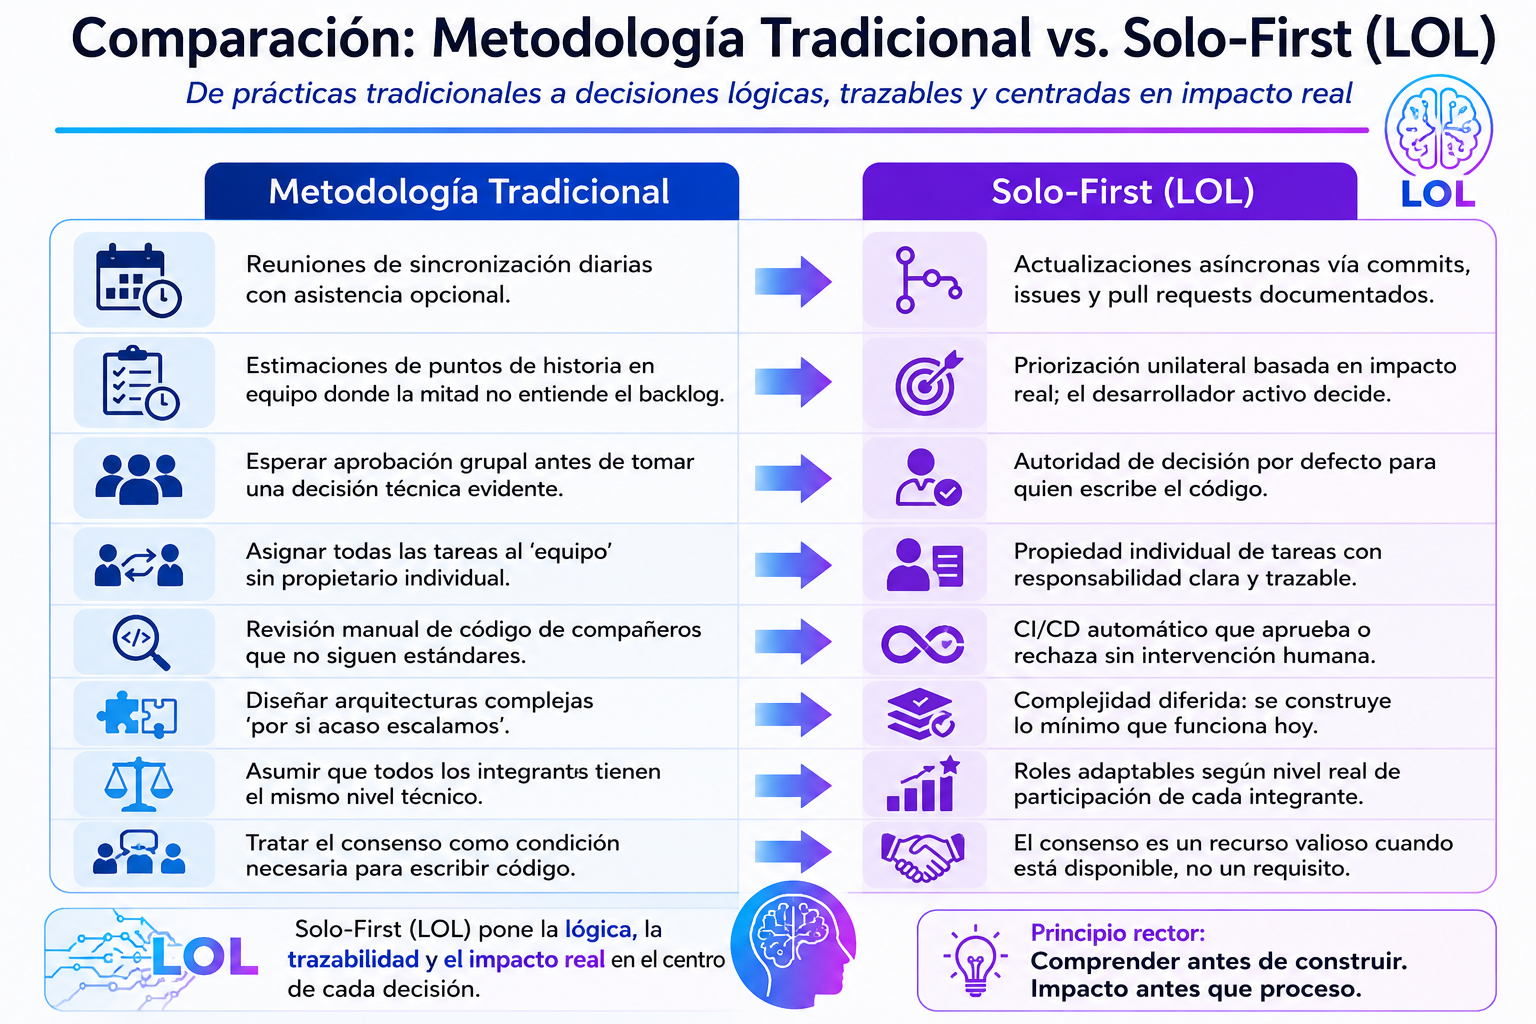
\includegraphics[width=0.95\linewidth]{imagenes/comparicionTradicional.png}
\caption{Comparacion:metodología tradicional vs Solo-First.}
\label{fig:lazy_framework}
\end{figure}


\section{III. Los 5 Valores Asimétricos}

El LOL Framework rediseña los cinco valores del desarrollo ágil clásico para la realidad del desarrollador asimétrico. No los descarta --- los adapta.



% --- In your document ---
\begin{table}[htbp]
\centering
\renewcommand{\arraystretch}{1.4} % CRITICAL: Gives 14pt text vertical breathing room
% \small % (Optional Pro-Tip: Uncomment this line if you want the table text to be one size smaller than the 14pt body text for better proportion)

\begin{tabularx}{\textwidth}{
    >{\raggedright\arraybackslash\hsize=0.9\hsize}X 
    >{\raggedright\arraybackslash\hsize=1.1\hsize}X
}
\toprule
\textbf{Agile Clásico dice\ldots} & \textbf{Solo-First dice\ldots} \\
\midrule
Individuos e interacciones sobre procesos y herramientas. & 
\textbf{Individuos activos} sobre interacciones vacías. Las herramientas automatizadas compensan las interacciones ausentes. \\
\addlinespace
Software funcionando sobre documentación exhaustiva. & 
Software funcionando sobre documentación exhaustiva. \textit{(Este lo mantenemos exactamente igual; era el correcto desde el principio.)} \\
\addlinespace
Colaboración con el cliente sobre negociación de contratos. & 
\textbf{Retroalimentación real} de la comunidad sobre suposiciones del equipo. El usuario final es el cliente más honesto. \\
\addlinespace
Respuesta al cambio sobre seguir un plan. & 
\textbf{Decisiones basadas en evidencia} sobre debates sin datos. El coraje técnico se construye sobre pruebas automatizadas, no sobre confianza ciega. \\
\addlinespace
Simplicidad: el arte de maximizar el trabajo no realizado. & 
\textbf{Simplicidad como escudo de supervivencia}. En solitario, el código que no escribiste no puede romperse ni necesitar mantenimiento. \\
\bottomrule
\end{tabularx}
\caption{Comparativa entre los principios de Agile Clásico y la metodología Solo-First.}
\label{tab:agile_vs_solo_first}
\end{table}


\section{IV. Una Nota para el Observador}

Si estás leyendo esto y no eres el desarrollador principal del proyecto, esta sección es para ti.



No eres un estorbo. No eres un problema que el framework tuvo que resolver. Eres una parte real del sistema, con un rol diseñado específicamente para lo que puedes contribuir.

El LOL Framework define cuatro niveles de participación porque la realidad de los equipos es diversa: algunas personas programan, otras documentan, otras validan, otras observan y reportan. Ninguno de estos niveles es inferior. Lo inferior es la ausencia total de contribución.



\begin{authorobservation}
\enquote{El Observador que escribe una buena bitácora del proceso, valida funcionalidades desde la perspectiva del usuario o documenta una decisión técnica compleja está contribuyendo tan realmente como el que escribe código. La diferencia es que su trabajo es visible de otras maneras.} — Capítulo 11 · Roles y Niveles de Participación · LOL Framework
\end{authorobservation}



Lo que el framework te pide, si decides asumir el rol de Observador:



Documenta el proceso con honestidad. Las decisiones tomadas, los problemas encontrados, las soluciones intentadas.

Valida el sistema desde afuera. Úsalo como un usuario real y reporta lo que no funciona como esperabas.

Mantén una perspectiva independiente. Tu valor no es estar de acuerdo con todo; es notar lo que el desarrollador, por estar demasiado adentro del código, no puede ver.

Produce tus artefactos con la misma seriedad con la que el desarrollador produce su código.



El Observador que cumple con esto tiene tanto para mostrar el día de la entrega como el desarrollador principal. Solo que en formatos distintos.



\section{V. La Firma}

Un manifiesto sin compromiso es solo un ensayo bien formateado. Esta es la parte donde el framework deja de ser filosofía y se convierte en práctica.



\begin{authorobservation}
Yo, como desarrollador Solo-First, me comprometo a: Avanzar sin paralizarme esperando participación que no llega. Construir sistemas simples, seguros y documentados. Diseñar mi proyecto para que otros puedan unirse sin que yo tenga que detenerme. Usar la automatización como árbitro neutral de calidad. Fallar rápido, aprender inmediatamente y seguir adelante. Respetar las contribuciones de todos los niveles de participación. Entregar un producto que responda a una necesidad real, no a una suposición.   Firma: \_\_\_\_\_\_\_\_\_\_\_\_\_\_\_\_\_\_\_\_\_\_\_\_\_\_\_\_\_\_\_\_     Fecha: \_\_\_\_\_\_\_\_\_\_\_\_\_\_\_\_
\end{authorobservation}





"El software evoluciona, las comunidades evolucionan

y las metodologías también deberían hacerlo."

--- Reflexión del Autor · LOL Framework

\begin{authorobservation}
LOL Framework · Solo-First · LAZY + LOL · 2026
\end{authorobservation}


\chapter{LAZY Framework}

\section{Definición}

LAZY (Listen, Analyze, Zoom, Yield) es un marco de investigación socio-tecnológica diseñado para transformar necesidades humanas, comunitarias u organizacionales en requisitos concretos para el desarrollo de soluciones tecnológicas.

Su propósito principal consiste en reducir la brecha existente entre la investigación social y la implementación técnica, proporcionando un proceso estructurado que permita identificar problemas relevantes, comprender sus causas y generar información accionable para equipos de desarrollo.

A diferencia de enfoques puramente académicos centrados en la producción de documentación, LAZY busca generar resultados que puedan ser utilizados directamente durante el diseño y construcción de sistemas de software.

El marco está compuesto por cuatro fases secuenciales: Listen, Analyze, Zoom y Yield.

\begin{figure}[htbp]
\centering
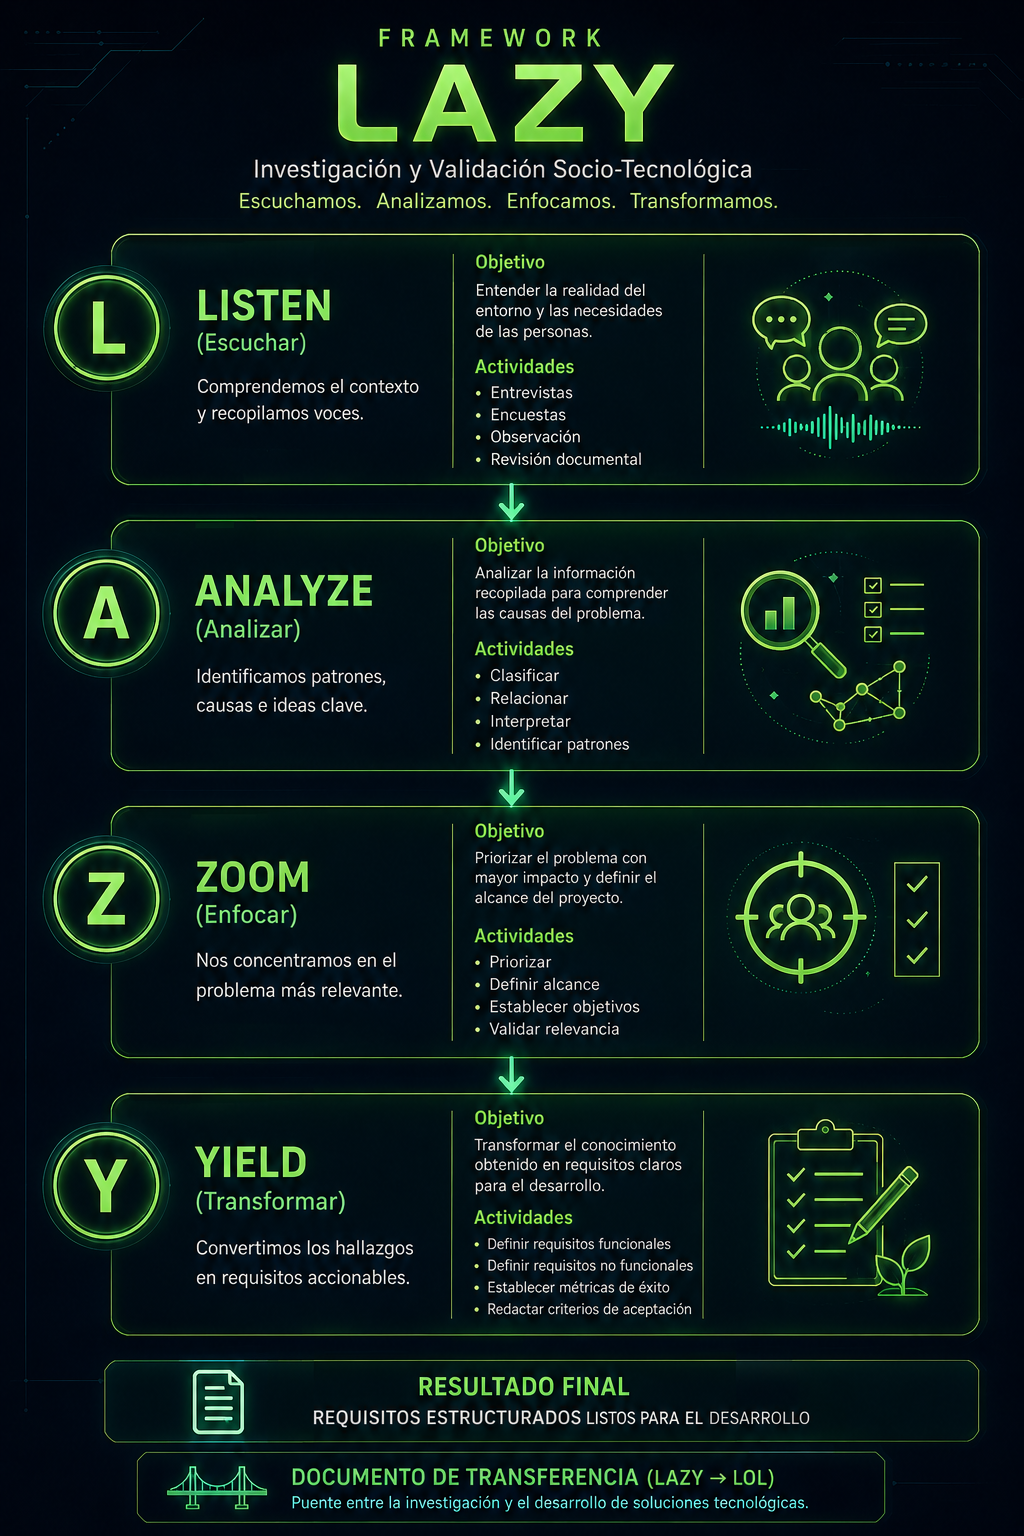
\includegraphics[width=0.85\linewidth]{imagenes/LAZY.png}
\caption{El Ciclo LAZY: Fases operativas para el diagnóstico e investigación de necesidades.}
\label{fig:lazy_cycle}
\end{figure}

\par\vspace{1.5em}\noindent\hfill\rule{0.25\textwidth}{0.6pt}\hfill\par\vspace{1.5em}

\section{Principios Fundamentales}

LAZY se fundamenta en los siguientes principios:

\subsection{Relevancia Social}

Toda iniciativa tecnológica debe responder a una necesidad real identificada dentro de una comunidad, organización o grupo de usuarios.

\subsection{Simplicidad Operativa}

El proceso de investigación debe concentrarse en obtener información útil para la toma de decisiones, evitando actividades que generen documentación excesiva sin aportar valor práctico.

\subsection{Evidencia sobre Suposiciones}

Las decisiones deben basarse en observaciones, entrevistas, encuestas o datos verificables, reduciendo la dependencia de percepciones subjetivas.

\subsection{Participación Suficiente}

Cada actividad debe involucrar únicamente el número de participantes necesario para alcanzar sus objetivos de manera efectiva.

La participación adicional puede aportar perspectivas complementarias, pero no constituye un requisito obligatorio para la validez del proceso.

Este principio reconoce que los equipos reales poseen diferentes niveles de disponibilidad, experiencia e interés, permitiendo una distribución flexible de responsabilidades sin comprometer la calidad de los resultados.

\par\vspace{1.5em}\noindent\hfill\rule{0.25\textwidth}{0.6pt}\hfill\par\vspace{1.5em}

\section{Fase L: Listen}

La fase Listen tiene como objetivo comprender la realidad del contexto estudiado.

Durante esta etapa se recopila información proveniente de usuarios, comunidades, organizaciones o grupos de interés mediante entrevistas, observaciones, encuestas o análisis documental.

La pregunta central de esta fase es:

\begin{keyquestion}
\enquote{¿Qué problema existe realmente?}
\end{keyquestion}

El resultado esperado es un inventario inicial de necesidades, dificultades y oportunidades identificadas dentro del entorno analizado.

\par\vspace{1.5em}\noindent\hfill\rule{0.25\textwidth}{0.6pt}\hfill\par\vspace{1.5em}

\section{Fase A: Analyze}

La fase Analyze busca transformar la información recopilada en conocimiento estructurado.

Durante esta etapa se identifican patrones, relaciones y causas comunes entre los problemas observados.

Las actividades pueden incluir clasificación de información, análisis de frecuencia, identificación de actores involucrados y evaluación de impacto.

La pregunta central de esta fase es:

\begin{keyquestion}
\enquote{¿Por qué ocurre este problema?}
\end{keyquestion}

El resultado esperado es una comprensión más profunda de las causas que generan la situación observada.

\par\vspace{1.5em}\noindent\hfill\rule{0.25\textwidth}{0.6pt}\hfill\par\vspace{1.5em}

\section{Fase Z: Zoom}

La fase Zoom se enfoca en reducir el alcance del problema a una dimensión manejable y técnicamente viable.

En numerosos proyectos se identifican múltiples necesidades simultáneamente. Sin embargo, intentar resolverlas todas suele conducir a soluciones complejas y difíciles de implementar.

Por esta razón, LAZY propone seleccionar el problema con mayor impacto potencial y concentrar los esfuerzos en dicho objetivo.

La pregunta central de esta fase es:

\begin{keyquestion}
\enquote{¿Qué problema debemos resolver primero?}
\end{keyquestion}

El resultado esperado es una definición clara del problema prioritario y de los límites del proyecto.

\par\vspace{1.5em}\noindent\hfill\rule{0.25\textwidth}{0.6pt}\hfill\par\vspace{1.5em}

\section{Fase Y: Yield}

La fase Yield representa la transición entre la investigación y el desarrollo.

Durante esta etapa los hallazgos obtenidos son transformados en requisitos funcionales, requisitos no funcionales, métricas de éxito y criterios de aceptación.

La pregunta central de esta fase es:

\begin{keyquestion}
\enquote{¿Cómo convertimos este conocimiento en una solución?}
\end{keyquestion}

El resultado esperado es un conjunto de requerimientos estructurados capaces de alimentar directamente el proceso de desarrollo dentro del marco LOL.

\par\vspace{1.5em}\noindent\hfill\rule{0.25\textwidth}{0.6pt}\hfill\par\vspace{1.5em}

\section{Entregables de LAZY}

Al finalizar el proceso, LAZY debe producir los siguientes elementos:

\begin{itemize}
\item Descripción del contexto estudiado.
\item Problemas identificados.
\item Análisis de causas.
\item Problema priorizado.
\item Objetivos del proyecto.
\item Requisitos iniciales.
\item Métricas de éxito.
\item Documento de transferencia hacia LOL.
\end{itemize}

Estos entregables constituyen la salida formal del marco y representan la entrada principal para las actividades de desarrollo de software.

\begin{authorobservation}
En una ocasión participé en un proyecto donde el equipo comenzó a proponer soluciones desde la primera reunión. Durante varios días discutimos tecnologías, bases de datos y diseños de interfaz. Sin embargo, nadie había hablado aún con los usuarios.

Cuando finalmente realizamos entrevistas, descubrimos que varias de nuestras ideas iniciales resolvían problemas que la comunidad nunca había mencionado. Aquella experiencia me enseñó que escuchar suele ser más eficiente que asumir. Parte de esa lección quedó reflejada posteriormente en la fase Listen de LAZY.
\end{authorobservation}



\chapter{LOL Framework}

\section{Definición}

LOL (Logic, Oversight, Layering) es un marco de desarrollo de software diseñado para transformar requisitos validados en soluciones tecnológicas funcionales, seguras y mantenibles.

Mientras que el marco LAZY se enfoca en comprender y estructurar problemas provenientes de contextos sociales u organizacionales, LOL se concentra en la construcción de la solución tecnológica correspondiente.

La propuesta de LOL surge de la observación de que numerosos proyectos académicos y profesionales enfrentan dificultades no únicamente durante la etapa de investigación, sino también durante la implementación técnica. Problemas relacionados con requisitos ambiguos, ausencia de supervisión, fallos de seguridad y distribución desigual de responsabilidades suelen afectar la calidad del producto final.

Con el objetivo de abordar estas situaciones, LOL organiza el desarrollo alrededor de tres pilares fundamentales: Logic, Oversight y Layering.

\begin{figure}[htbp]
\centering
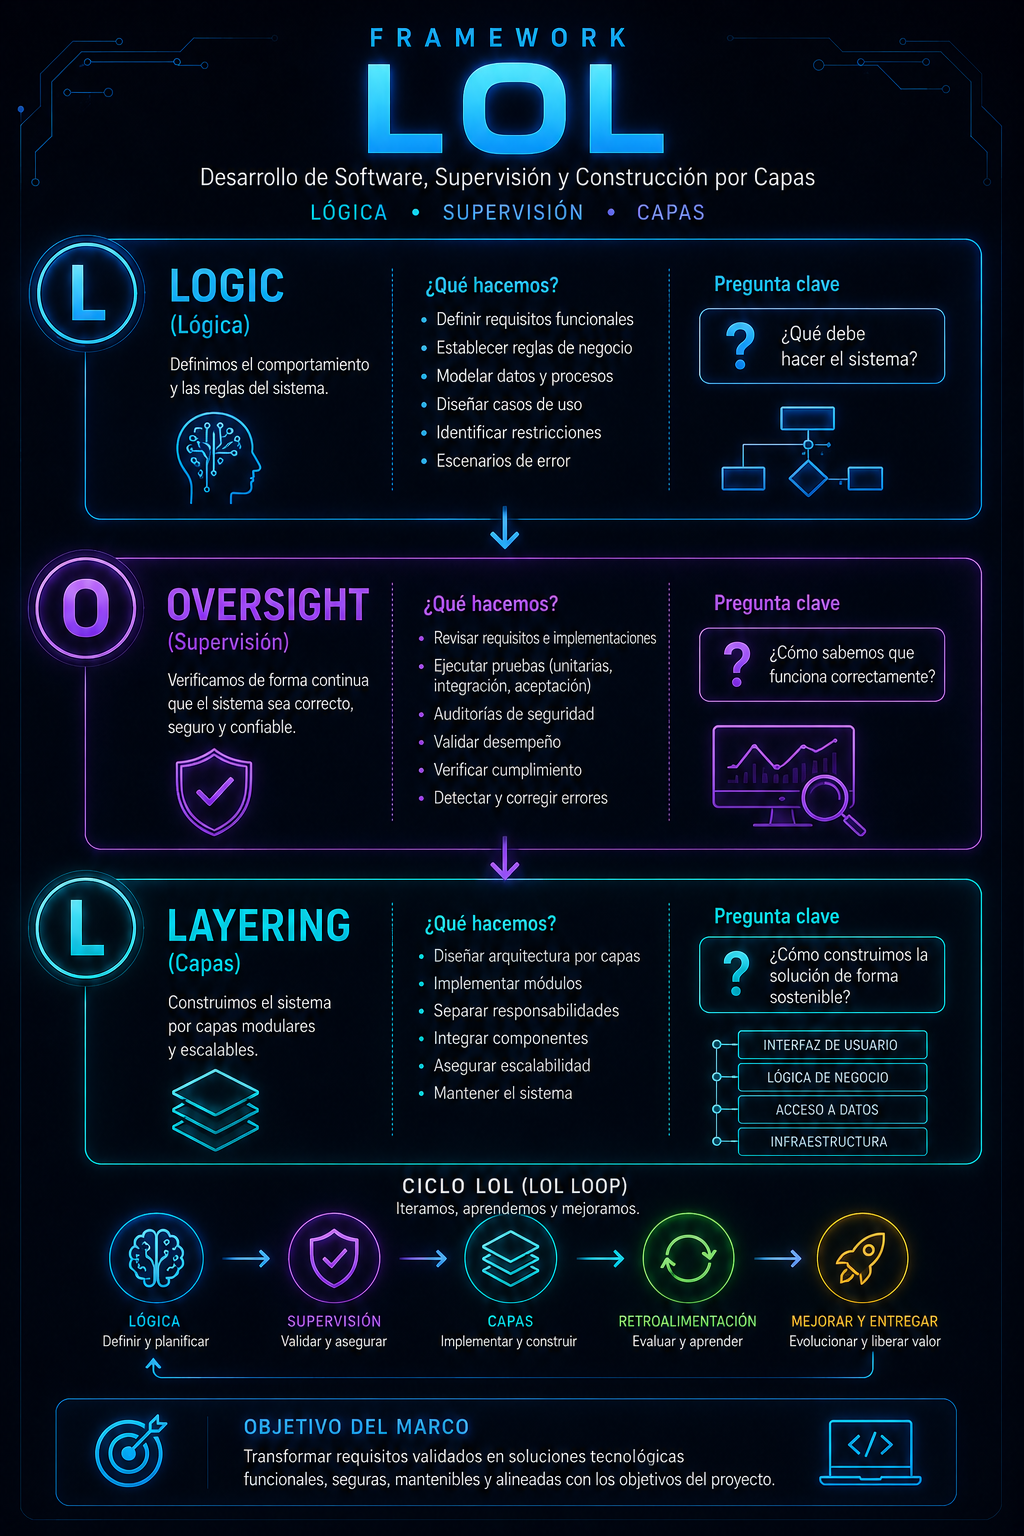
\includegraphics[width=0.85\linewidth]{imagenes/LOL.png}
\caption{El Framework LOL: Logic, Oversight y Layering como pilares del desarrollo asimétrico.}
\label{fig:lol_framework}
\end{figure}

\par\vspace{1.5em}\noindent\hfill\rule{0.25\textwidth}{0.6pt}\hfill\par\vspace{1.5em}

\section{Principios Fundamentales}

\subsection{La lógica antes que el código}

Antes de implementar cualquier funcionalidad, debe existir una comprensión clara de las reglas, restricciones y objetivos del sistema.

LOL considera que numerosos errores de software no son consecuencia de una mala programación, sino de una definición insuficiente de la lógica del problema.

\subsection{Supervisión continua}

La calidad no debe verificarse únicamente al final del proyecto.

Las actividades de revisión, validación y control deben realizarse de forma continua durante todo el ciclo de desarrollo.

\subsection{Construcción por capas}

Los sistemas deben diseñarse considerando múltiples niveles de protección, responsabilidad y organización.

Cada capa debe cumplir una función específica dentro de la arquitectura general.

\subsection{Participación adaptable}

Los equipos reales poseen distintos niveles de experiencia, disponibilidad y especialización.

Por esta razón, LOL permite distribuir responsabilidades según las capacidades y aportes efectivos de cada participante, manteniendo la continuidad del proyecto incluso cuando la participación no es uniforme.

\par\vspace{1.5em}\noindent\hfill\rule{0.25\textwidth}{0.6pt}\hfill\par\vspace{1.5em}

\section{Pilar L: Logic}

Logic representa la definición formal del comportamiento esperado del sistema.

Durante esta etapa se establecen:

\begin{itemize}
\item Requisitos funcionales.
\item Reglas de negocio.
\item Restricciones operativas.
\item Modelos de datos.
\item Casos de uso.
\item Escenarios de error.
\end{itemize}

La pregunta central es:

\begin{keyquestion}
\enquote{¿Qué debe hacer el sistema?}
\end{keyquestion}

El objetivo consiste en construir una fuente única de verdad que sirva como referencia para todas las etapas posteriores del desarrollo.

\par\vspace{1.5em}\noindent\hfill\rule{0.25\textwidth}{0.6pt}\hfill\par\vspace{1.5em}

\section{Pilar O: Oversight}

Oversight representa los mecanismos de supervisión y control de calidad.

Durante esta etapa se realizan actividades de:

\begin{itemize}
\item Revisión de requisitos.
\item Validación de implementaciones.
\item Pruebas funcionales.
\item Auditorías de seguridad.
\item Evaluación de desempeño.
\item Verificación de cumplimiento.
\end{itemize}

La pregunta central es:

\begin{keyquestion}
\enquote{¿Cómo sabemos que funciona correctamente?}
\end{keyquestion}

A diferencia de modelos donde las pruebas se concentran al final del proyecto, LOL incorpora supervisión continua durante todo el proceso de desarrollo.

\par\vspace{1.5em}\noindent\hfill\rule{0.25\textwidth}{0.6pt}\hfill\par\vspace{1.5em}

\section{Pilar L: Layering}

Layering representa la construcción estructurada de la solución tecnológica.

El sistema es dividido en componentes, módulos o capas con responsabilidades claramente definidas.

Entre ellas pueden encontrarse:

\begin{itemize}
\item Interfaz de usuario.
\item Lógica de negocio.
\item Persistencia de datos.
\item Seguridad.
\item Integraciones externas.
\end{itemize}

La pregunta central es:

\begin{keyquestion}
\enquote{¿Cómo construimos la solución de manera sostenible?}
\end{keyquestion}

Este enfoque facilita el mantenimiento, la escalabilidad y la evolución futura del sistema.

\par\vspace{1.5em}\noindent\hfill\rule{0.25\textwidth}{0.6pt}\hfill\par\vspace{1.5em}

\section{Ciclo LOL}

LOL opera mediante ciclos iterativos denominados LOL Loops.

Cada ciclo sigue la secuencia:

Logic → Oversight → Layering → Retroalimentación

Durante cada iteración se define una parte del sistema, se valida su calidad y posteriormente se implementa dentro de la arquitectura general.

Los resultados obtenidos generan nueva información que alimenta el siguiente ciclo.

Este mecanismo permite una evolución progresiva del producto sin perder control sobre la calidad o la coherencia técnica.

\par\vspace{1.5em}\noindent\hfill\rule{0.25\textwidth}{0.6pt}\hfill\par\vspace{1.5em}

\section{Objetivo del Marco}

El objetivo principal de LOL no es reemplazar metodologías existentes ni competir directamente con marcos consolidados como Scrum, Kanban o XP.

Su propósito consiste en proporcionar una estructura adaptable que permita transformar requisitos previamente validados en soluciones tecnológicas funcionales, manteniendo un equilibrio entre simplicidad, supervisión y organización arquitectónica.

Dentro de la arquitectura propuesta en este trabajo, LOL constituye el mecanismo de resolución tecnológica que complementa el proceso de investigación desarrollado mediante LAZY.

\begin{authorobservation}
Como estudiante de Ingeniería de Software, muchas veces sentí la tentación de abrir el editor y comenzar a programar inmediatamente. Programar es divertido. Documentar reglas, analizar restricciones o revisar requisitos suele ser menos emocionante.

Sin embargo, algunos de los errores más costosos que encontré no fueron errores de programación, sino errores de comprensión. El sistema funcionaba exactamente como había sido construido, pero no como debía funcionar. Por esa razón, LOL propone que la lógica preceda al código y no al revés.
\end{authorobservation}




\chapter{Roles y Niveles de Participación}

\section{Introducción}

Existe una tendencia frecuente en los marcos tradicionales de desarrollo a asumir que todos los integrantes de un equipo participarán de manera similar durante todo el proyecto. Aunque esta premisa resulta razonable desde una perspectiva organizacional, la experiencia práctica demuestra que la realidad suele ser más diversa.

Algunas personas destacan por sus capacidades técnicas. Otras poseen habilidades de comunicación, análisis o documentación. Algunas disponen de más tiempo. Otras participan de manera ocasional debido a responsabilidades académicas, laborales o personales.

LOL parte de una observación sencilla: la participación no siempre es uniforme, pero eso no significa que sea inexistente.

Por esta razón, el marco introduce una estructura flexible basada en roles y niveles de participación, permitiendo que los integrantes contribuyan de acuerdo con sus capacidades, disponibilidad y contexto.

\begin{figure}[htbp]
\centering
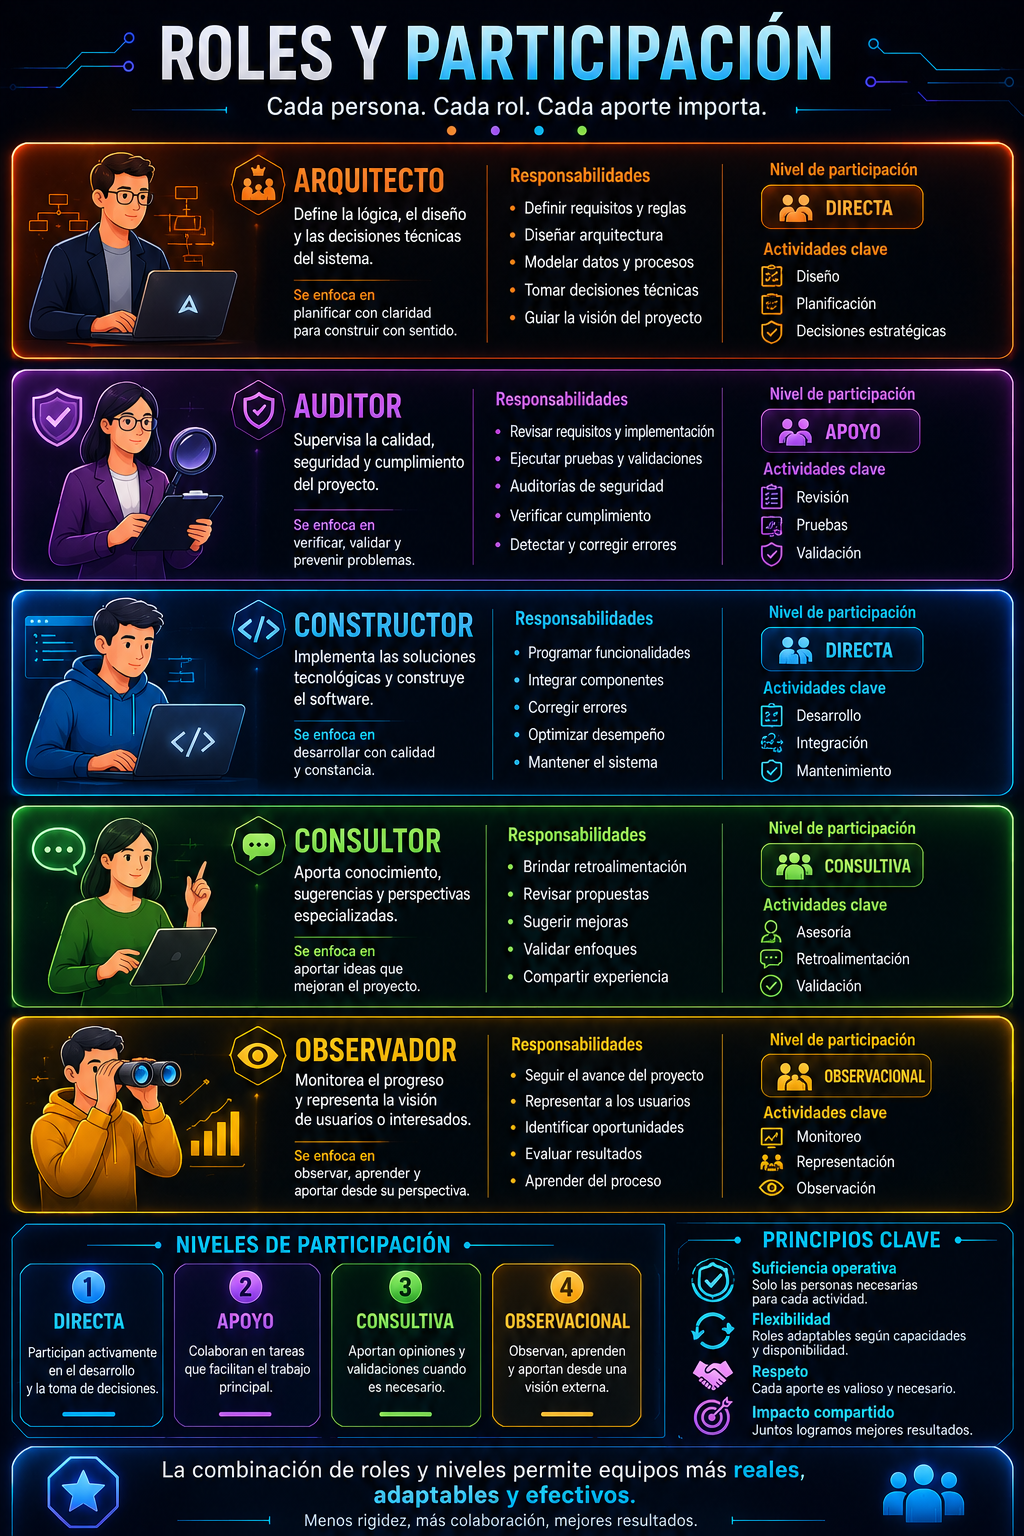
\includegraphics[width=0.85\linewidth]{imagenes/rolesYParticipacio.png}
\caption{Niveles de Participación Adaptativa y su correspondencia con los Roles de Desarrollo.}
\label{fig:roles_participacion}
\end{figure}

\par\vspace{1.5em}\noindent\hfill\rule{0.25\textwidth}{0.6pt}\hfill\par\vspace{1.5em}

\section{Principio de Participación Adaptativa}

LOL adopta el Principio de Participación Adaptativa.

Este principio establece que los miembros de un equipo no están obligados a contribuir mediante las mismas actividades ni con la misma intensidad.

Lo importante no es que todos realicen exactamente las mismas tareas, sino que cada rol aporte valor al objetivo común del proyecto.

Bajo esta perspectiva, la efectividad del equipo no se mide únicamente por la cantidad de trabajo realizado por cada integrante, sino por la capacidad colectiva para alcanzar los resultados esperados.

\par\vspace{1.5em}\noindent\hfill\rule{0.25\textwidth}{0.6pt}\hfill\par\vspace{1.5em}

\section{Niveles de Participación}

LOL define cuatro niveles generales de participación.

\subsection{Nivel 1: Participación Directa}

Corresponde a los integrantes que ejecutan actividades fundamentales para la construcción de la solución.

Ejemplos:

\begin{itemize}
\item Programación.
\item Diseño arquitectónico.
\item Investigación principal.
\item Implementación de funcionalidades.
\end{itemize}

Estos participantes suelen asumir la mayor responsabilidad técnica dentro del proyecto.

\par\vspace{1.5em}\noindent\hfill\rule{0.25\textwidth}{0.6pt}\hfill\par\vspace{1.5em}

\subsection{Nivel 2: Participación de Apoyo}

Incluye actividades que facilitan el trabajo principal sin intervenir directamente en la implementación.

Ejemplos:

\begin{itemize}
\item Documentación.
\item Organización de información.
\item Preparación de presentaciones.
\item Gestión de requisitos.
\end{itemize}

Su contribución mejora la eficiencia y trazabilidad del proyecto.

\par\vspace{1.5em}\noindent\hfill\rule{0.25\textwidth}{0.6pt}\hfill\par\vspace{1.5em}

\subsection{Nivel 3: Participación Consultiva}

Corresponde a integrantes que aportan observaciones, sugerencias o validaciones periódicas.

Ejemplos:

\begin{itemize}
\item Revisión de propuestas.
\item Retroalimentación sobre prototipos.
\item Verificación de requisitos.
\item Evaluación de entregables.
\end{itemize}

Aunque su participación es menos frecuente, puede influir significativamente en la calidad de las decisiones.

\par\vspace{1.5em}\noindent\hfill\rule{0.25\textwidth}{0.6pt}\hfill\par\vspace{1.5em}

\subsection{Nivel 4: Participación Observacional}

Incluye participantes cuya función principal consiste en seguir el avance del proyecto y proporcionar perspectivas externas cuando sea necesario.

Estos participantes pueden actuar como observadores, usuarios piloto o representantes de grupos de interés.

Su objetivo no es dirigir el proyecto ni intervenir constantemente, sino contribuir a mantener una visión independiente sobre los resultados obtenidos.

\par\vspace{1.5em}\noindent\hfill\rule{0.25\textwidth}{0.6pt}\hfill\par\vspace{1.5em}

\section{Roles dentro de LOL}

Los roles representan responsabilidades funcionales y no cargos jerárquicos.

Un mismo participante puede asumir múltiples roles dependiendo del tamaño y las necesidades del equipo.

\subsection{Arquitecto}

Responsable de definir la lógica fundamental del sistema.

Sus funciones incluyen:

\begin{itemize}
\item Diseño conceptual.
\item Definición de requisitos.
\item Modelado de datos.
\item Toma de decisiones técnicas.
\end{itemize}

\par\vspace{1.5em}\noindent\hfill\rule{0.25\textwidth}{0.6pt}\hfill\par\vspace{1.5em}

\subsection{Auditor}

Responsable de supervisar la calidad y consistencia del proyecto.

Sus funciones incluyen:

\begin{itemize}
\item Revisión de entregables.
\item Verificación de requisitos.
\item Pruebas y validaciones.
\item Supervisión de seguridad.
\end{itemize}

\par\vspace{1.5em}\noindent\hfill\rule{0.25\textwidth}{0.6pt}\hfill\par\vspace{1.5em}

\subsection{Constructor}

Responsable de implementar la solución tecnológica.

Sus funciones incluyen:

\begin{itemize}
\item Desarrollo de software.
\item Integración de componentes.
\item Corrección de errores.
\item Mantenimiento técnico.
\end{itemize}

\par\vspace{1.5em}\noindent\hfill\rule{0.25\textwidth}{0.6pt}\hfill\par\vspace{1.5em}

\subsection{Observador}

Responsable de aportar perspectivas externas y retroalimentación independiente.

Sus funciones incluyen:

\begin{itemize}
\item Revisión general del proyecto.
\item Validación de objetivos.
\item Identificación de problemas visibles.
\item Evaluación desde la perspectiva del usuario.
\end{itemize}

\par\vspace{1.5em}\noindent\hfill\rule{0.25\textwidth}{0.6pt}\hfill\par\vspace{1.5em}

\section{Equipos de Participación Variable}

LOL reconoce que distintos proyectos requieren diferentes configuraciones de equipo.

Por ejemplo:

Un proyecto pequeño podría funcionar adecuadamente con una sola persona desempeñando simultáneamente los roles de Arquitecto, Constructor y Auditor.

Un proyecto académico de tres integrantes podría distribuir los roles entre un participante principal y dos observadores o colaboradores consultivos.

Un proyecto profesional podría asignar múltiples personas a cada rol.

La estructura propuesta no busca imponer una composición específica, sino proporcionar un mecanismo flexible capaz de adaptarse a distintas realidades organizacionales.

\par\vspace{1.5em}\noindent\hfill\rule{0.25\textwidth}{0.6pt}\hfill\par\vspace{1.5em}

\section{Principio de Suficiencia Operativa}

No todas las tareas requieren la participación de todos los integrantes.

LOL establece que una actividad debe involucrar únicamente la cantidad de participantes necesaria para alcanzar sus objetivos de manera efectiva.

Cuando una tarea puede ser realizada adecuadamente por una persona, no existe una obligación metodológica de involucrar a cinco.

Cuando una actividad requiere múltiples perspectivas, la participación adicional se convierte en una ventaja.

El objetivo no consiste en maximizar la cantidad de participantes por tarea, sino maximizar el valor generado por cada participación.

\begin{authorobservation}
Durante un proyecto universitario observé que dos integrantes del equipo participaban de forma muy limitada. Mi reacción inicial fue considerar la situación como un problema organizacional. Sin embargo, al analizar el trabajo realizado, descubrí algo más interesante: muchas tareas habían sido completadas por una sola persona porque la naturaleza de esas actividades no requería más participantes.

Esto me llevó a cuestionar una idea que consideraba evidente: que todos los miembros de un equipo deben participar siempre de la misma manera y con la misma intensidad. A partir de esa experiencia surgieron los conceptos de Participación Adaptativa y Suficiencia Operativa, que posteriormente fueron incorporados al framework LOL.
\end{authorobservation}



\chapter{Integración entre LAZY y LOL}

\section{Introducción}

Hasta este punto se han presentado dos marcos complementarios: LAZY, orientado a la investigación socio-tecnológica, y LOL, orientado al desarrollo de soluciones tecnológicas.

Sin embargo, el valor principal de la propuesta no reside únicamente en la existencia de ambos marcos de forma independiente, sino en la relación que existe entre ellos.

Mientras LAZY busca comprender un problema, LOL busca resolverlo.

Mientras LAZY genera conocimiento, LOL genera soluciones.

Por esta razón, ambos marcos forman parte de una arquitectura integrada cuyo propósito es transformar necesidades reales en sistemas funcionales.

\par\vspace{1.5em}\noindent\hfill\rule{0.25\textwidth}{0.6pt}\hfill\par\vspace{1.5em}

\section{El Problema de la Desconexión}

En numerosos proyectos académicos y profesionales existe una separación significativa entre la fase de investigación y la fase de implementación.

Los equipos suelen realizar entrevistas, encuestas, observaciones y análisis que posteriormente son documentados en informes extensos. Sin embargo, la transición entre dichos resultados y el desarrollo de software no siempre es clara.

Como consecuencia, pueden aparecer situaciones como:

\begin{itemize}
\item Requisitos ambiguos.
\item Interpretaciones incorrectas.
\item Funcionalidades innecesarias.
\item Pérdida de información relevante.
\item Soluciones técnicamente correctas pero socialmente irrelevantes.
\end{itemize}

Esta situación genera una brecha entre lo que las personas necesitan y lo que finalmente se construye.

La integración entre LAZY y LOL busca reducir dicha brecha.

\par\vspace{1.5em}\noindent\hfill\rule{0.25\textwidth}{0.6pt}\hfill\par\vspace{1.5em}

\section{Flujo General de Integración}

La relación entre ambos marcos puede entenderse como un flujo continuo de transformación.

LAZY recibe como entrada una realidad social o problemática observada.

A través de sus fases de investigación, análisis y priorización, produce un conjunto de hallazgos estructurados.

Posteriormente, estos hallazgos son entregados a LOL en forma de requisitos, objetivos y criterios de éxito.

LOL utiliza esta información como punto de partida para diseñar, validar e implementar la solución tecnológica correspondiente.

De esta manera, cada decisión técnica mantiene una conexión directa con una necesidad previamente identificada.

\par\vspace{1.5em}\noindent\hfill\rule{0.25\textwidth}{0.6pt}\hfill\par\vspace{1.5em}

\section{El Documento de Transferencia}

La principal conexión formal entre ambos marcos es el Documento de Transferencia.

Este documento representa la salida de LAZY y la entrada de LOL.

Su contenido incluye:

\begin{itemize}
\item Descripción del problema.
\item Contexto de la investigación.
\item Usuarios involucrados.
\item Objetivos identificados.
\item Requisitos funcionales.
\item Requisitos no funcionales.
\item Restricciones conocidas.
\item Métricas de éxito.
\end{itemize}

La finalidad de este documento es asegurar que la información obtenida durante la investigación pueda ser utilizada directamente durante el desarrollo.

\par\vspace{1.5em}\noindent\hfill\rule{0.25\textwidth}{0.6pt}\hfill\par\vspace{1.5em}

\section{Del Problema a la Solución}

La integración puede describirse mediante una secuencia de transformación progresiva:

Problema observado

↓

Necesidad identificada

↓

Problema priorizado

↓

Objetivos definidos

↓

Requisitos estructurados

↓

Diseño técnico

↓

Implementación

↓

Solución funcional

Cada transición reduce la incertidumbre y aumenta el nivel de definición del proyecto.

En este sentido, LAZY y LOL no representan procesos separados, sino diferentes etapas de una misma cadena de creación de valor.

\par\vspace{1.5em}\noindent\hfill\rule{0.25\textwidth}{0.6pt}\hfill\par\vspace{1.5em}

\section{Retroalimentación Continua}

Aunque la integración principal ocurre cuando LAZY entrega información a LOL, la relación entre ambos marcos no es completamente unidireccional.

Durante el desarrollo pueden surgir descubrimientos técnicos, limitaciones operativas o nuevas necesidades que requieran revisar hipótesis previamente establecidas.

Cuando esto ocurre, LOL puede generar retroalimentación hacia LAZY.

Esta comunicación bidireccional permite actualizar requisitos, redefinir prioridades y mejorar la comprensión del problema original.

La arquitectura resultante se comporta como un sistema de aprendizaje continuo.

\par\vspace{1.5em}\noindent\hfill\rule{0.25\textwidth}{0.6pt}\hfill\par\vspace{1.5em}

\section{Beneficios de la Integración}

La integración entre LAZY y LOL proporciona diversas ventajas:

\begin{itemize}
\item Reduce la distancia entre investigación y desarrollo.
\item Mejora la trazabilidad de los requisitos.
\item Facilita la toma de decisiones.
\item Incrementa la relevancia social de las soluciones desarrolladas.
\item Disminuye el riesgo de implementar funcionalidades innecesarias.
\item Mantiene la conexión entre objetivos sociales y objetivos técnicos.
\end{itemize}

Además, permite que proyectos socio-tecnológicos sean abordados mediante una estructura coherente desde la identificación del problema hasta la entrega de la solución.

\par\vspace{1.5em}\noindent\hfill\rule{0.25\textwidth}{0.6pt}\hfill\par\vspace{1.5em}

\section{Visión General de la Arquitectura}

La propuesta presentada en este trabajo puede resumirse de la siguiente manera:

LAZY identifica y estructura el problema.

LOL diseña y construye la solución.

La integración entre ambos garantiza que cada componente tecnológico tenga una justificación basada en evidencia obtenida durante la investigación.

De esta forma, la arquitectura LAZY-LOL busca proporcionar un recorrido completo desde la comprensión de una necesidad hasta la generación de una respuesta tecnológica capaz de producir un impacto real.

\begin{figure}[htbp]
\centering
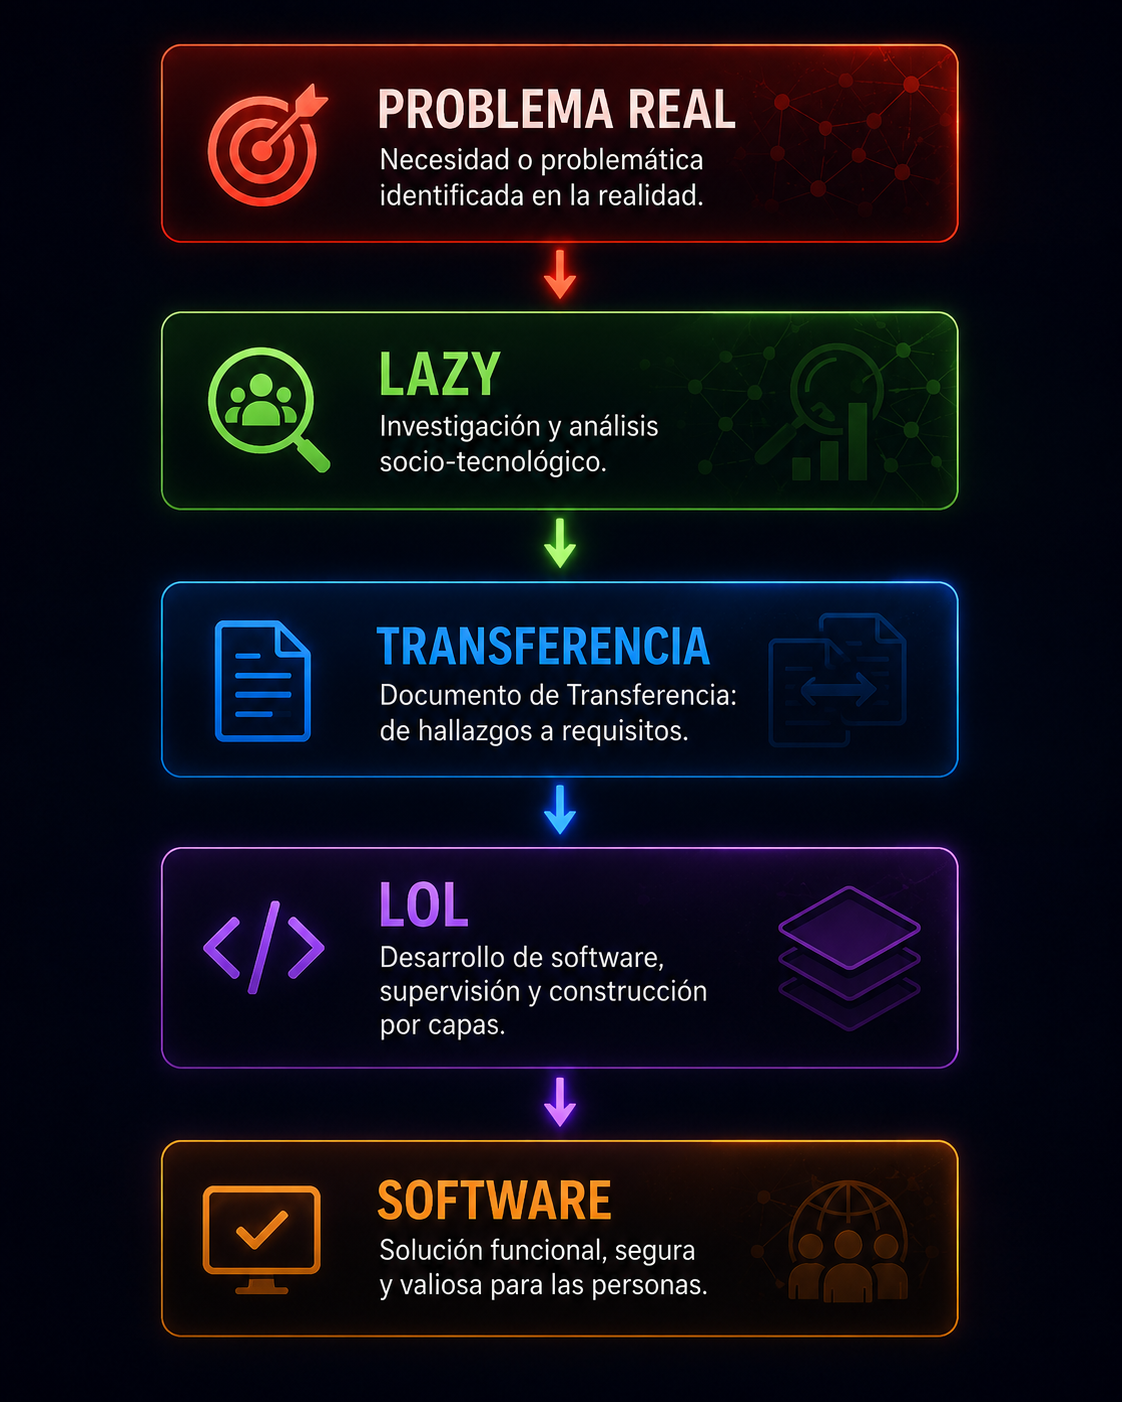
\includegraphics[width=0.85\linewidth]{imagenes/transferenciaLAZYLOL.png}
\caption{Arquitectura Integrada LAZY-LOL: Flujo bidireccional desde la investigación social hasta la entrega de la solución tecnológica.}
\label{fig:arquitectura_integrada}
\end{figure}



\chapter{Caso de Estudio: Sistema de Información Web para la Comunidad La Barranca}

\section{Introducción}

El presente capítulo documenta la aplicación de la arquitectura metodológica LAZY-LOL en el desarrollo del Sistema de Información Web (SIW) para el Consejo Comunal La Barranca (CC La Barranca), proyecto de carácter socio-tecnológico desarrollado en el contexto de un programa universitario de Ingeniería de Software.

A diferencia de ejemplos simplificados utilizados frecuentemente en entornos académicos ---como aplicaciones de gestión de tareas o calculadoras de escritorio--- el presente caso involucra una comunidad real con necesidades específicas, usuarios con diferentes niveles de alfabetización digital, un sistema de roles organizacional pre-existente y restricciones técnicas derivadas del contexto de despliegue. Por esta razón, constituye un escenario representativo para evaluar la viabilidad y aplicabilidad de los marcos propuestos en condiciones reales de trabajo.

El código fuente completo del sistema se encuentra disponible en el repositorio público: github.com/gmoralesm-dev/CC-La-Barranca. Este capítulo conecta las decisiones de diseño observables en dicho repositorio con los principios y fases de LAZY y LOL descritos en capítulos anteriores.

\section{Contexto del Proyecto}

El Consejo Comunal La Barranca es una organización comunitaria de base que gestiona información, recursos y comunicaciones para un grupo de familias residentes en su área de influencia. Su estructura organizacional interna incluye roles diferenciados: Administrador, Vocera Principal y Líderes de Calle, quienes tienen responsabilidades distintas en la gestión de la información comunitaria.

Antes del desarrollo del sistema, la comunidad operaba mediante procesos manuales o parcialmente digitalizados para actividades como la difusión de anuncios, el registro de familias, la emisión de constancias y certificados, y la gestión de entregas de recursos. Estos procesos presentaban dificultades documentadas de acceso, trazabilidad y coordinación entre los distintos roles organizacionales.

El equipo de desarrollo estuvo compuesto por tres integrantes universitarios, con una distribución de participación asimétrica que reproduce exactamente el escenario descrito en el planteamiento del problema de este trabajo: un desarrollador principal con participación de Nivel 1 (Directa) y dos colaboradores con participación de Nivel 3 y 4 respectivamente (Consultiva y Observacional).

\section{Aplicación del Framework LAZY}

\subsection{Fase L: Listen — Escucha del Contexto Comunitario}

La fase Listen consistió en el contacto directo con integrantes del Consejo Comunal para comprender sus necesidades operativas reales. Se realizaron entrevistas informales con la Vocera Principal y dos Líderes de Calle, orientadas a identificar las tareas que actualmente resultaban más difíciles, lentas o propensas a error en su gestión cotidiana.

Los hallazgos principales de esta fase pueden resumirse en cuatro categorías de necesidades:

Difusión de información: Los anuncios comunitarios se distribuían por grupos de WhatsApp, lo que generaba pérdida de información histórica y dificultad para llegar a habitantes sin smartphone o con datos limitados.

Registro de familias: El padrón de familias y sus miembros se mantenía en documentos físicos o archivos Excel, sin control de versiones ni acceso compartido.

Certificados y constancias: La emisión de documentos certificados por la comunidad requería procesos manuales de impresión, firma y entrega presencial, sin registro digital de los documentos emitidos.

Gestión de entregas: Los eventos de distribución de recursos (alimentos, materiales) carecían de registro sistemático, dificultando la trazabilidad de beneficiarios y cantidades.



\subsection{Fase A: Analyze — Análisis y Patrones}

Durante la fase Analyze se procesó la información recolectada para identificar patrones comunes. El análisis reveló que todos los problemas identificados compartían una causa raíz: la ausencia de una fuente única de verdad digital accesible para los diferentes roles del Consejo Comunal. Cada proceso operaba con su propia isla de información, sin integración ni trazabilidad entre ellas.

Adicionalmente, el análisis de actores permitió identificar tres perfiles de usuarios con necesidades distintas: gestores operativos (Vocera Principal y Líderes de Calle) que necesitan acceso de escritura para administrar información, miembros de la comunidad que necesitan acceso de lectura para consultar anuncios y verificar documentos, y visitantes ocasionales que requieren acceso mínimo sin registro permanente.

Esta diferenciación de actores se convertiría directamente en el sistema de roles implementado en la fase LOL.



\subsection{Fase Z: Zoom — Focalización del Alcance}

La fase Zoom resultó crítica para evitar la trampa habitual de los proyectos socio-tecnológicos: intentar resolver todos los problemas identificados simultáneamente. Se aplicó el criterio de mayor impacto con menor complejidad técnica inicial para seleccionar el conjunto de funcionalidades del Producto Mínimo Viable (MVP).

El problema priorizado fue: la ausencia de un canal centralizado, accesible y permanente para la gestión de información comunitaria. Las funcionalidades seleccionadas para el primer ciclo de desarrollo fueron: tablón de comunicados público, registro de familias, emisión de certificados digitales y registro de entregas. La gestión de reportes y la arquitectura de roles avanzada quedaron definidas como funcionalidades de ciclos posteriores.



\subsection{Fase Y: Yield — Transferencia hacia LOL}

La fase Yield produjo el Documento de Transferencia que conectó formalmente la investigación social con el desarrollo técnico. Este documento definió los requisitos funcionales del sistema, los perfiles de usuario con sus permisos correspondientes, y las métricas de éxito que el sistema debía cumplir para ser considerado exitoso desde la perspectiva comunitaria.

Los elementos clave del Documento de Transferencia que informaron directamente la Fase Logic de LOL fueron:



\begin{table}[htbp]
\centering
\begin{tabular}{p{0.28\textwidth} p{0.32\textwidth} p{0.35\textwidth}}
\toprule
\textbf{Hallazgo LAZY} & \textbf{Requisito técnico generado} & \textbf{Implementación en LOL} \\
\midrule
Anuncios se pierden en WhatsApp & Módulo de comunicados persistente con lectura pública & Colección /comunicados con allow read: if true \\
Padrón de familias en Excel no compartido & CRUD de familias con control de acceso por rol & Colección /families con isManager() para escritura \\
Certificados emitidos sin registro & Generación de PDF con persistencia en BD & Módulo jsPDF + colección /certificates \\
Distribución de recursos sin trazabilidad & Registro de eventos de entrega con historial & Colección /deliveries con timestamps de servidor \\
Tres perfiles de usuarios con permisos distintos & Sistema de roles jerárquico verificado en servidor & Función getUserRole() + función isManager() \\
Visitantes ocasionales sin registro permanente & Sesiones de acceso temporal sin cuenta permanente & Colección /invitados con sesiones de Firebase Auth \\
\bottomrule
\end{tabular}
\end{table}



\section{Aplicación del Framework LOL}

\subsection{Stack Tecnológico}

\begin{table}[htbp]
\centering
\renewcommand{\arraystretch}{1.4} % Gives 14pt text vertical breathing room
\small % Makes table text slightly smaller for better proportion

% Standard tabular with fixed-width columns (no extra packages needed)
\begin{tabular}{p{0.45\textwidth} p{0.45\textwidth}}
\hline
\textbf{Agile Clásico dice\ldots} & \textbf{Solo-First dice\ldots} \\
\hline
Individuos e interacciones sobre procesos y herramientas. & 
\textbf{Individuos activos} sobre interacciones vacías. Las herramientas automatizadas compensan las interacciones ausentes. \\
\hline
Software funcionando sobre documentación exhaustiva. & 
Software funcionando sobre documentación exhaustiva. \textit{(Este lo mantenemos exactamente igual; era el correcto desde el principio.)} \\
\hline
Colaboración con el cliente sobre negociación de contratos. & 
\textbf{Retroalimentación real} de la comunidad sobre suposiciones del equipo. El usuario final es el cliente más honesto. \\
\hline
Respuesta al cambio sobre seguir un plan. & 
\textbf{Decisiones basadas en evidencia} sobre debates sin datos. El coraje técnico se construye sobre pruebas automatizadas, no sobre confianza ciega. \\
\hline
Simplicidad: el arte de maximizar el trabajo no realizado. & 
\textbf{Simplicidad como escudo de supervivencia}. En solitario, el código que no escribiste no puede romperse ni necesitar mantenimiento. \\
\hline
\end{tabular}

\caption{Comparativa entre los principios de Agile Clásico y la metodología Solo-First.}
\label{tab:agile_vs_solo_first_case_study}
\end{table}

El sistema fue construido con el siguiente stack tecnológico, seleccionado bajo el principio de Complejidad Diferida de LOL: tecnologías maduras, bien documentadas y con el menor overhead de configuración posible para un equipo reducido con tiempo académico limitado.

\begin{table}[htbp]
\centering
\small % CRITICAL: Reduces table text to ~12pt to balance the 14pt body text
\renewcommand{\arraystretch}{1.4} % Adds vertical breathing room

\begin{tabularx}{\textwidth}{
    >{\raggedright\arraybackslash\hsize=0.7\hsize}X % Tecnología + Versión (Narrow)
    >{\raggedright\arraybackslash\hsize=1.3\hsize}X % Rol en el Sistema (Wider)
    >{\raggedright\arraybackslash\hsize=1.0\hsize}X % Pilar LOL (Medium)
}
\toprule
\textbf{Tecnología} & \textbf{Rol en el Sistema} & \textbf{Pilar LOL} \\
\midrule

\texttt{React} \newline \footnotesize{(v19.1.0)} & 
Interfaz de usuario y lógica de presentación. & 
Layering — UI \\
\addlinespace

\texttt{Firebase Auth} \newline \footnotesize{(v10.12.3)} & 
Autenticación y gestión de sesiones. & 
Layering — Autenticación \\
\addlinespace

\texttt{Firebase Firestore} \newline \footnotesize{(v10.12.3)} & 
Base de datos NoSQL en tiempo real. & 
Layering — Persistencia \\
\addlinespace

\texttt{Firebase Hosting} & 
Despliegue de la aplicación web. & 
Layering — Infraestructura \\
\addlinespace

\texttt{Firestore Rules v2} & 
Control de acceso declarativo en servidor. & 
Oversight — Seguridad \\
\addlinespace

\texttt{html2canvas + jsPDF} \newline \footnotesize{(v1.4.1 / 3.0)} & 
Generación de certificados PDF. & 
Layering — Certificados \\
\addlinespace

% --- LÍNEA CORREGIDA AQUÍ ---
\texttt{@testing-}\allowbreak\texttt{library} \newline \footnotesize{(v16.3.0)} & 
Suite de pruebas unitarias de UI. & 
Oversight — Validación \\
\addlinespace
% ----------------------------

\texttt{.env.example} & 
Gestión segura de credenciales (anti-hardcoding). & 
Logic — Configuración \\

\bottomrule
\end{tabularx}
\caption{Stack tecnológico seleccionado bajo el principio de Complejidad Diferida.}
\label{tab:stack_tecnologico}
\end{table}

\subsection{Pilar L: Logic — Definición de la Lógica del Sistema}

La Fase Logic estableció las reglas fundamentales del sistema antes de escribir código funcional. El artefacto central de esta fase fue la definición del esquema de datos de Firestore y la especificación del sistema de roles, derivados directamente del Documento de Transferencia de LAZY.

El sistema organiza toda su información bajo la colección raíz Consejo-Comunal-La-Barranca, con ocho subcolecciones funcionales que reflejan los módulos operativos del Consejo Comunal:






Una decisión de diseño significativa de la Fase Logic fue la arquitectura del sistema de roles. En lugar de almacenar los roles en el token de autenticación del cliente ---donde podrían ser manipulados--- se optó por persistirlos en la base de datos del servidor y consultarlos desde las Security Rules mediante la función getUserRole(). Esta decisión mitiga directamente la amenaza de Elevation of Privilege (E) del modelo STRIDE.


\begin{tcolorbox}[
    colback=primary!5,
    colframe=primary!30,
    arc=5pt,
    title=Ejemplo simplificado de validación de roles
]

\begin{verbatim}
function getUserRole() {
    return user.role;
}

function isManager() {
    return auth != null &&
           role in {
               "administrador",
               "admin",
               "lider_de_calle",
               "vocera_principal"
           };
}
\end{verbatim}

\smallskip
\textit{
Ejemplo simplificado. La implementación real depende
de la plataforma utilizada y puede consultarse en el repositorio del proyecto.
}

\end{tcolorbox}

\subsection{Pilar O: Oversight — Supervisión y Control de Seguridad}

El Pilar Oversight del sistema se implementó principalmente a través de las Firebase Security Rules, que actúan como la capa de control de acceso declarativa en el servidor. Estas reglas constituyen el artefacto de Oversight más crítico del sistema: son verificadas por Firebase antes de permitir cualquier operación de lectura o escritura, independientemente de la lógica implementada en el cliente React.

El análisis de amenazas STRIDE aplicado durante la Fase Logic produjo las siguientes mitigaciones, todas implementadas y verificables en el archivo firestore.rules del repositorio:



\begin{table}[htbp]
\centering
\begin{tabular}{p{0.18\textwidth} p{0.25\textwidth} p{0.35\textwidth} p{0.16\textwidth}}
\toprule
\textbf{Amenaza STRIDE} & \textbf{Vector Identificado} & \textbf{Mitigación Implementada} & \textbf{Artefacto} \\
\midrule
S — Spoofing & Usuario no autenticado accede a datos de familias & Firebase Auth obligatorio en todas las rutas protegidas; regla: request.auth != null & firestore.rules L.32 \\
T — Tampering & Usuario modifica su propio rol a 'administrador' & getUserRole() consulta el rol desde la BD del servidor, nunca desde el cliente o token & firestore.rules L.7–9 \\
R — Repudiation & Administrador niega haber emitido un certificado & Colección certificates con timestamps de servidor; logs de Firestore habilitados & Colección /certificates \\
I — Info. Disclosure & Usuario estándar lee datos de otras familias por ID directo (IDOR) & Queries de families siempre scoped por autenticación; roles verificados en servidor & firestore.rules L.31–44 \\
D — Denial of Service & Registros masivos de comunicados por usuario anónimo & allow write: if request.auth != null en comunicados; comentarios requieren auth & firestore.rules L.24–30 \\
E — Elevation of Privilege & Usuario intenta autoasignarse rol de lider\_de\_calle & isManager() verifica roles desde BD; escritura de users solo sobre propio UID & firestore.rules L.10–17, L.47 \\
\bottomrule
\end{tabular}
\end{table}



Adicionalmente, el proyecto configura una suite de pruebas de interfaz mediante @testing-library/react, que permite la validación automatizada del comportamiento de los componentes de UI. Esta suite cumple la función de Oversight continuo descrita en el Ciclo LOL: cada cambio en la interfaz puede ser verificado contra el comportamiento esperado antes de ser desplegado.



\subsection{Pilar L: Layering — Construcción por Capas}

El Pilar Layering organizó el sistema en capas con responsabilidades claramente definidas, siguiendo el principio de separación de responsabilidades establecido en la Fase Logic:



\begin{table}[htbp]
\centering
\begin{tabular}{p{0.22\textwidth} p{0.24\textwidth} p{0.24\textwidth} p{0.25\textwidth}}
\toprule
\textbf{Capa} & \textbf{Responsabilidad} & \textbf{Tecnología} & \textbf{Principio LOL} \\
\midrule
Presentación & Interfaz de usuario, formularios, navegación & React 19 + CSS & Complejidad Diferida: UI simple y funcional primero \\
Lógica de Aplicación & Gestión de estado, validaciones del cliente, generación de PDF & React Hooks + html2canvas + jsPDF & Validación doble: cliente y servidor \\
Autenticación & Sesiones de usuario, tokens, roles & Firebase Auth & Confianza cero en el cliente: roles verificados en servidor \\
Persistencia & Almacenamiento y consulta de datos en tiempo real & Firebase Firestore & Colecciones separadas por dominio funcional \\
Control de Acceso & Políticas declarativas de lectura y escritura & Firestore Security Rules v2 & Oversight continuo: reglas independientes del cliente \\
Infraestructura & Despliegue, hosting, variables de entorno & Firebase Hosting + .env & Credenciales fuera del código fuente (.env.example) \\
\bottomrule
\end{tabular}
\end{table}



Una decisión de Layering destacable es el manejo de credenciales. El repositorio incluye un archivo .env.example que documenta las variables de entorno requeridas sin exponer valores reales, y el .gitignore excluye explícitamente los archivos .env del control de versiones. Esta práctica, recomendada en el Capítulo 5 de este trabajo como responsabilidad del Sentry, previene la exposición de credenciales de Firebase en repositorios públicos.



\section{Roles y Niveles de Participación}

\subsection{Roles del Sistema (Perspectiva Técnica)}

El sistema implementa cinco roles funcionales derivados directamente de la estructura organizacional del Consejo Comunal, mapeados a los niveles de participación del LOL Framework:



\begin{table}[htbp]
\centering
\begin{tabular}{p{0.22\textwidth} p{0.24\textwidth} p{0.24\textwidth} p{0.25\textwidth}}
\toprule
\textbf{Rol del Sistema} & \textbf{Permiso de Lectura} & \textbf{Permiso de Escritura} & \textbf{Nivel LOL} \\
\midrule
Público (sin auth) & comunicados solamente & Ninguno & Nivel 4 — Observacional \\
Invitado (invitados) & Solo su sesión propia & Solo su sesión propia & Nivel 4 — Observacional \\
Usuario autenticado & comunicados, families, deliveries, certificates, reports & comunicados y comentarios propios & Nivel 3 — Consultivo \\
lider\_de\_calle & Todo lo anterior & families, members, receipts, deliveries, certificates, reports & Nivel 2 — Apoyo \\
vocera\_principal & Todo lo anterior & Todo lo anterior & Nivel 1 — Directo \\
administrador / admin & Todo lo anterior & Todo lo anterior + gestión de usuarios & Nivel 1 — Directo \\
\bottomrule
\end{tabular}
\end{table}



Esta tabla demuestra una correspondencia directa entre el modelo de participación adaptativa de LOL y la estructura de permisos del sistema real: los roles con mayor responsabilidad en la comunidad tienen mayor capacidad de escritura en el sistema, y los roles observacionales tienen acceso de lectura o sesiones temporales.

\subsection{Roles del Equipo de Desarrollo (Perspectiva Metodológica)}

La distribución de participación observada en el equipo de desarrollo durante el proyecto reflejó con precisión el escenario descrito en el Principio Solo-First del LOL Framework:



\begin{table}[htbp]
\centering
\begin{tabular}{p{0.22\textwidth} p{0.24\textwidth} p{0.24\textwidth} p{0.25\textwidth}}
\toprule
\textbf{Integrante} & \textbf{Rol LOL Asumido} & \textbf{Nivel de Participación} & \textbf{Contribuciones Principales} \\
\midrule
Desarrollador principal & Arquitecto + Constructor + Auditor & Nivel 1 — Directa & Diseño de arquitectura, implementación de todos los módulos, configuración de Firestore Rules, despliegue en Firebase Hosting \\
Colaborador 2 & Observador (parcial) & Nivel 3 — Consultivo & Retroalimentación sobre la interfaz de usuario, validación de flujos desde la perspectiva del usuario comunitario \\
Colaborador 3 & Observador & Nivel 4 — Observacional & Documentación del proceso, seguimiento de avances, preparación de material de presentación \\
\bottomrule
\end{tabular}
\end{table}



Esta distribución, aunque asimétricamente inclinada hacia el desarrollador principal, fue gestionada mediante los mecanismos del LOL Framework sin que la falta de participación uniforme bloqueara el avance del proyecto. Las decisiones técnicas fueron tomadas unilateralmente bajo el principio de Dictador por Defecto, mientras los colaboradores aportaron desde sus niveles de participación reales.




\begin{table}[htbp]
\centering
\begin{tabular}{p{0.28\textwidth} p{0.32\textwidth} p{0.35\textwidth}}
\toprule
\textbf{Métrica} & \textbf{Valor} & \textbf{Relevancia en LOL} \\
\midrule
Módulos funcionales implementados & 8 colecciones Firestore + UI correspondiente & Pilar Layering completado en Loop 1 \\
Reglas de seguridad (firestore.rules) & 79 líneas, 6 colecciones principales protegidas & Pilar Oversight — cobertura completa de acceso \\
Roles del sistema implementados & 6 roles (público, invitado, usuario, 3 managers) & Logic — sistema de roles verificado en servidor \\
Amenazas STRIDE mitigadas en diseño & 6/6 (S, T, R, I, D, E) & Logic — análisis de amenazas preventivo completo \\
Archivos de test configurados & Suite @testing-library configurada & Oversight — base de validación automatizada \\
Credenciales expuestas en repositorio & 0 (solo .env.example con placeholders) & Layering — seguridad de configuración correcta \\
Tecnologías de terceros integradas & 7 (React, Firebase x4, jsPDF, html2canvas) & Complejidad Diferida: mínimas y bien justificadas \\
\bottomrule
\end{tabular}
\end{table}






\section{Lecciones Aprendidas}

\subsection{Sobre la Integración LAZY-LOL}

La principal lección aprendida durante el proyecto fue la confirmación empírica del valor del Documento de Transferencia como artefacto de integración. En la práctica, este documento evitó que la fase de desarrollo comenzara con requisitos ambiguos: cada decisión técnica ---desde la elección de colecciones en Firestore hasta el diseño del sistema de roles--- tenía una justificación directamente trazable a un hallazgo de la fase LAZY.

Sin este mecanismo de transferencia, la tendencia natural habría sido comenzar el desarrollo con supuestos sobre las necesidades de la comunidad, lo que probablemente habría resultado en funcionalidades técnicamente correctas pero socialmente irrelevantes.

\subsection{Sobre el Principio Solo-First en la Práctica}

La experiencia confirmó que el diseño Solo-First no es una concesión a la falta de colaboración, sino una decisión arquitectónica que protege la calidad del proyecto en condiciones de participación variable. El hecho de que el desarrollador principal pudiera tomar decisiones técnicas sin necesidad de consenso grupal fue determinante para mantener la coherencia técnica del sistema.

Al mismo tiempo, la \enquote{Docking Station} conceptual del framework funcionó en la práctica: los colaboradores pudieron contribuir desde sus niveles de participación reales sin necesitar comprender la arquitectura completa del sistema, y sus aportaciones (retroalimentación de UI, documentación, seguimiento) fueron formalizadas como artefactos verificables del proceso.

\subsection{Sobre la Seguridad por Diseño}

El análisis STRIDE aplicado en la Fase Logic demostró ser más eficiente que las revisiones de seguridad post-desarrollo. Identificar durante el diseño que los roles debían verificarse desde el servidor ---y no confiar en el token del cliente--- evitó una vulnerabilidad de Elevation of Privilege que habría sido significativamente más costosa de corregir después de que el código funcional ya estuviera escrito.

Esta experiencia respalda empíricamente uno de los principios centrales de LOL Framework: la seguridad como propiedad emergente del diseño, no como corrección posterior.

\begin{authorobservation}
La lección más importante del proyecto La Barranca no es técnica: es que comprender correctamente un problema comunitario —con sus roles, sus procesos y sus limitaciones reales— es tan determinante para el éxito del sistema como la calidad del código que lo implementa. LAZY no es burocracia académica; es la diferencia entre construir lo correcto y construir correctamente lo incorrecto.
\end{authorobservation}






\chapter{Del Campo al Marco Teórico: Reinterpretación del SIW-CC bajo los Frameworks LOL y LAZY}

\section{Introducción: El Problema con XP (o con cómo la contamos)}

El Sistema de Información Web para el CC La Barranca fue desarrollado oficialmente bajo la metodología Extreme Programming (XP). Esta declaración es técnicamente correcta, académicamente aceptable y metodológicamente... incompleta.

XP describe con precisión las prácticas de codificación empleadas: iteraciones cortas, historias de usuario, pruebas continuas, cliente presente. Lo que XP no describe ---porque no fue diseñado para hacerlo--- es la dinámica real detrás de un equipo asimétrico: quién levantó los requerimientos, quién tomó las decisiones de arquitectura, quién escribió el código cuando el equipo no estaba disponible y quién, al final del día, era el único con contexto completo del sistema.

Este capítulo propone una relectura del mismo proyecto bajo dos frameworks complementarios: LOL (Logic-Oversight-Layering) como metodología de desarrollo de software, y LAZY (Listen-Analyze-Zoom-Yield) como metodología de investigación. El argumento central es el siguiente:

LOL y LAZY no contradicen lo que ocurrió en el proyecto. Lo describen con mayor fidelidad.

Lo que sigue no es una revisión histórica ficticia. Es una demostración de que los eventos documentados en las Partes I--IV de este informe ---las entrevistas, las decisiones de arquitectura, las iteraciones de código--- encajan de forma natural y precisa dentro de los principios de LOL y LAZY, y que dicha correspondencia no es casual: es la evidencia de que ambos frameworks emergen de la práctica real, no del papel.



\section{La Fase de Investigación como Instancia de LAZY}

LAZY es un acrónimo que describe el proceso de investigación situacional en cinco fases: Listen (escuchar), Analyze (analizar), Zoom (enfocar), Yield (producir). Su premisa fundamental es que el investigador que trabaja en condiciones asimétricas ---con acceso limitado a colaboradores, con una comunidad que no habla el lenguaje técnico--- necesita un proceso de recolección de información que sea riguroso sin ser rígido.

La Parte I y II del informe del SIW-CC documentan, sin saberlo, una implementación textual de LAZY.



\subsection{Fase L — Listen (Escuchar)}

El primer contacto con el CC La Barranca no fue una encuesta ni un formulario de requerimientos. Fue una conversación. Los autores visitaron la comunidad, se sentaron con la Vocera Principal y los cuatro Líderes de Calle, y los dejaron hablar.

Lo que escucharon no fue una especificación técnica. Fue una narrativa de frustraciones: \enquote{los cuadernos se pierden}, \enquote{no sabemos cuántas familias hay exactamente}, \enquote{la gente no sabe cuándo es la entrega}. Esta escucha activa es exactamente la fase L de LAZY: recolección sin filtro, sin agenda previa, sin formularios que limiten las respuestas.

El instrumento documentado en el Marco Metodológico ---el Guión de Entrevista semi-estructurado con \enquote{temas a explorar} en lugar de preguntas cerradas--- es el artefacto que materializa la fase Listen. No se buscaba confirmar hipótesis. Se buscaba entender el mundo como lo vive la comunidad.



\subsection{Fase A — Analyze (Analizar)}

Una vez recolectada la información de campo, los investigadores la procesaron mediante dos herramientas de modelado visual: el Árbol de Problemas y el Árbol de Objetivos (Gráficos 2 y 3 del informe original).

Estos diagramas son la fase A de LAZY en acción. No son decorativos. Son el resultado del análisis cualitativo que identificó causas raíz (registro manual, ausencia de SIW, falta de capacitación) y efectos observables (pérdida de información, comunidad desinformada, desconfianza en los procesos).

La tabla de evaluación cuantitativa (Cuadro 4) que priorizó el Problema 4 sobre los demás no es una decisión arbitraria: es el output de aplicar criterios de análisis sobre los datos recolectados en la fase anterior. Analyze produce un ranking de realidad, no de preferencias.



\subsection{Fase Z — Zoom (Enfocar)}

De los cuatro problemas identificados, el proceso de análisis convergió en uno: la ausencia de un Sistema de Información Web. Esto es la fase Zoom: la transición del problema difuso (\enquote{el CC tiene problemas}) al problema accionable (\enquote{el CC necesita un SIW con estas funcionalidades específicas}).

El artefacto que documenta este enfoque son las 15 Historias de Usuario (HU1--HU15). Cada una define con precisión quirúrgica qué necesita cada tipo de actor, en qué contexto y con qué propósito. La suma de las historias es el modelo completo de la solución requerida. No hay ambigüedad, no hay scope creep: hay un conjunto delimitado de necesidades priorizadas.

Zoom también se manifiesta en la selección de alternativas (Cuadro 6): entre tres opciones (SIW, red social comunitaria, capacitación), el análisis multicriterio señaló al SIW como la solución con mayor impacto tecnológico y mejor factibilidad. Este no fue un juicio de gusto. Fue el resultado de aplicar criterios a datos.



\subsection{Fase Y — Yield (Producir)}

La fase Yield es el momento en que la investigación deja de ser investigación y se convierte en insumo para el desarrollo. En LAZY, el Documento de Transferencia es el artefacto que formaliza este cruce: todo lo que la investigación descubrió se empaqueta en un formato que el desarrollador (que en equipos asimétricos puede ser el mismo investigador) puede consumir directamente.

En el SIW-CC, este documento de transferencia existe implícitamente: es la consolidación del diagnóstico, las historias de usuario y el diseño de la base de datos NoSQL (colecciones families, members, deliveries, receipts, users) que se convirtió en el esquema arquitectónico del sistema. La transferencia de LAZY a LOL ocurrió en el Día 1 de la Iteración 0, cuando el equipo transformó las historias en decisiones técnicas concretas.



Cuadro 14.1 --- Correspondencia entre las fases LAZY y los artefactos del SIW-CC

\begin{table}[htbp]
\centering
\begin{tabular}{p{0.22\textwidth} p{0.24\textwidth} p{0.24\textwidth} p{0.25\textwidth}}
\toprule
\textbf{Fase LAZY} & \textbf{Descripción} & \textbf{Artefacto en el SIW-CC} & \textbf{Sección del Informe} \\
\midrule
L — Listen & Escucha activa sin agenda & Guión de entrevista semi-estructurado, notas de campo & Marco Metodológico \\
A — Analyze & Modelado de causas y efectos & Árbol de Problemas, Árbol de Objetivos, Cuadro 4 & Parte I \\
Z — Zoom & Convergencia en el problema accionable & 15 Historias de Usuario, Cuadro 6 de alternativas & Marco Metodológico / Parte I \\
Y — Yield & Producción del insumo para desarrollo & Esquema de BD Firestore, Diseño UX/UI, Casos de uso & Parte II / III \\
\bottomrule
\end{tabular}
\end{table}





\section{El Proceso de Desarrollo como Instancia de LOL}

LOL es el framework de desarrollo que gobierna cómo se construye software en condiciones de asimetría de equipo. Sus tres fases ---Logic, Oversight, Layering--- no son etapas secuenciales en el sentido tradicional. Son dimensiones que coexisten en cada iteración, con distinto peso según el momento del ciclo.

Las 18 jornadas de desarrollo documentadas en las Fases y Tiempos de Desarrollo del SIW-CC constituyen un caso de estudio que permite observar las tres fases de LOL operando simultáneamente.



\subsection{Fase Logic — La Arquitectura como Decisión Deliberada}

La fase Logic en LOL no es simplemente \enquote{planificación}. Es la construcción del modelo mental que permite tomar decisiones técnicas sin depender de consenso externo. En equipos simétricos, este modelo se construye en grupo. En equipos asimétricos, lo construye quien tiene contexto.

En la Iteración 0 (Días 1--4), las decisiones de la fase Logic quedaron documentadas con inusual claridad:

React.js como frontend: velocidad de prototipado, componentes reutilizables, ecosistema maduro.

Firebase (Firestore + Auth) como backend: autenticación segura sin gestionar servidor, base de datos en tiempo real, plan gratuito suficiente para el volumen del CC.

Arquitectura SPA: experiencia fluida para usuarios con conectividad variable.

Tailwind CSS: diseño responsivo sin CSS personalizado, adaptable a teléfonos y computadoras.

Estas no son elecciones técnicas triviales. Son expresiones de la fase Logic: cada decisión tiene una justificación que responde a las restricciones reales del contexto (conectividad intermitente, usuarios con baja alfabetización digital, presupuesto cero). La fase Logic de LOL exige que el desarrollador pueda articular por qué cada componente del sistema existe, no solo que funcione.

El Diagrama de Casos de Uso (Gráfico 19) es el artefacto central de la fase Logic: modela los actores (Vocera Principal, Líder de Calle, Firestore), sus responsabilidades y las relaciones entre módulos. Es el mapa que hace navegable el sistema antes de que exista una sola línea de código.



\subsection{Fase Oversight — La Seguridad como Evidencia de Responsabilidad}

La fase Oversight en LOL corresponde a la revisión crítica del sistema: ¿qué puede salir mal? ¿quién tiene acceso a qué? ¿los datos sensibles están protegidos? Esta fase es especialmente relevante en sistemas comunitarios donde se almacena información personal de familias vulnerables.

El SIW-CC implementó Oversight en múltiples capas, todas documentadas en el código fuente del repositorio público CC-La-Barranca:



\begin{table}[htbp]
\centering
\begin{tabular}{p{0.28\textwidth} p{0.32\textwidth} p{0.35\textwidth}}
\toprule
\textbf{Mecanismo de Oversight} & \textbf{Implementación Técnica} & \textbf{Amenaza Mitigada} \\
\midrule
Control de acceso por roles & Función getUserRole() consulta el rol desde Firestore server-side, nunca desde el cliente & Elevation of Privilege \\
Reglas de seguridad Firestore & families requiere auth para leer; solo managers para escribir & Acceso no autorizado a datos del censo \\
Aislamiento de documentos de usuario & users accede únicamente a su propio documento & IDOR (Insecure Direct Object Reference) \\
Comunicados de lectura pública & comunicados sin restricción de lectura & Asimetría de información comunitaria \\
Autenticación Firebase Auth & Verificación de identidad antes de cualquier operación de escritura & Suplantación de identidad \\
Sin credenciales en repositorio & Variables de entorno para config de Firebase & Exposición de secretos en código fuente \\
\bottomrule
\end{tabular}
\end{table}



Esta tabla no es una adición al proyecto original. Está construida directamente desde las Firestore Security Rules del repositorio. La fase Oversight de LOL no requiere que el desarrollador hable de seguridad en abstracto: requiere que el sistema lo demuestre en concreto.

Cabe señalar que ninguna de estas decisiones de seguridad fue discutida en las sesiones de planificación de XP documentadas en el informe original. Fueron tomadas de forma autónoma por el desarrollador principal, en silencio, sin comité. Esto es precisamente lo que LOL nomina como Oversight individual: la responsabilidad de revisar el propio trabajo con ojo crítico cuando no hay un equipo que lo haga por ti.



\subsection{Fase Layering — La Construcción Incremental como Principio}

Layering es la fase de LOL que describe cómo se construye funcionalidad sobre funcionalidad de forma deliberada: primero la base (autenticación, navegación, roles), luego el núcleo (gestión de familias y miembros), luego las capacidades derivadas (eventos de entrega, reportes, generación de constancias).

El Layering en el SIW-CC es explícito en la documentación de las iteraciones:



\begin{table}[htbp]
\centering
\begin{tabular}{p{0.22\textwidth} p{0.24\textwidth} p{0.24\textwidth} p{0.25\textwidth}}
\toprule
\textbf{Iteración} & \textbf{Días} & \textbf{Capa LOL} & \textbf{Funcionalidades Entregadas} \\
\midrule
Iteración 0 & 1–4 & Cimiento (Auth + Arquitectura) & Login, gestión de sesión, navegación por pestañas, lógica de roles isManagerRole \\
Iteración 1 & 5–10 & Núcleo (Datos primarios) & FamilyManagement.js: CRUD completo de familias; MemberManagement.js: gestión de núcleo familiar \\
Iteración 2 & 11–15 & Lógica de negocio (Operaciones) & DeliveryEvents.js: eventos de entrega; registro de beneficios; Reports.js: estadísticas en tiempo real \\
Iteración 3 & 16–18 & Valor agregado (Outputs) & CertificateGenerator.js: constancias de recepción; pulido UI con TailwindCSS; pruebas de aceptación \\
\bottomrule
\end{tabular}
\end{table}



La secuencia no es arbitraria. Si se hubiera intentado construir el generador de constancias en la Iteración 0, habría fallado porque no existía aún la colección de familias ni el modelo de eventos de entrega. El Layering en LOL no es solo un principio de buena práctica: es una restricción lógica que el desarrollador autónomo debe gestionar sin la red de seguridad de un equipo que detecte dependencias rotas.

La refactorización mencionada en la documentación del Día 8 ---\enquote{FamilyManagement.js estaba creciendo mucho}--- es también una expresión de Layering: la capacidad de reconocer cuándo una capa necesita ser reorganizada antes de que el peso de la complejidad la vuelva inmanejable.



Cuadro 14.2 --- Correspondencia entre las fases LOL y los artefactos del SIW-CC

\begin{table}[htbp]
\centering
\begin{tabular}{p{0.22\textwidth} p{0.24\textwidth} p{0.24\textwidth} p{0.25\textwidth}}
\toprule
\textbf{Fase LOL} & \textbf{Principio Central} & \textbf{Artefacto en el SIW-CC} & \textbf{Días de Desarrollo} \\
\midrule
Logic & Modelo mental explícito antes de codificar & Diagrama de Casos de Uso, decisiones de arquitectura documentadas, selección justificada del stack & 1–4 \\
Oversight & Revisión crítica autónoma de calidad y seguridad & Firestore Security Rules, getUserRole() server-side, pruebas de integración y UAT con Vocera & Transversal \\
Layering & Construcción incremental con dependencias respetadas & 3 iteraciones con capas explícitas: Auth → CRUD → Business Logic → Outputs & 5–18 \\
\bottomrule
\end{tabular}
\end{table}





\section{XP vs LOL+LAZY: No una Contradicción, sino una Ampliación}

Una objeción razonable a este capítulo es la siguiente: si el proyecto ya usaba XP y funcionó, ¿para qué reinterpretarlo bajo LOL y LAZY? La respuesta no es que XP estuviera equivocado. Es que XP describe el qué, mientras que LOL y LAZY describen el cómo y el por qué en contextos que XP no fue diseñado para contemplar.



\begin{table}[htbp]
\centering
\begin{tabular}{p{0.28\textwidth} p{0.32\textwidth} p{0.35\textwidth}}
\toprule
\textbf{Dimensión} & \textbf{XP (Extreme Programming)} & \textbf{LOL + LAZY} \\
\midrule
Contexto de equipo & Equipo simétrico, colaborativo, comunicación constante & Equipos asimétricos; roles opcionales (Spectator); avance autónomo posible \\
Rol del cliente & Cliente presente en todo momento, co-define prioridades & Cliente consultado en puntos clave (Listen + Yield); el desarrollador puede avanzar con criterio propio entre consultas \\
Gestión de seguridad & Buena práctica implícita, no prescriptiva & Oversight como fase explícita y obligatoria en cada iteración \\
Proceso de investigación & No contemplado (XP asume requerimientos conocidos) & LAZY provee el método para descubrir requerimientos cuando el cliente no sabe articularlos \\
Documentación de decisiones & Minimizada (\enquote{código sobre documentación}) & Logic exige que las decisiones de arquitectura sean articulables y justificables \\
Aplicabilidad académica & Requiere adaptar terminología al contexto universitario & Diseñado desde el inicio para contextos académicos con dinámicas de evaluación institucional \\
\bottomrule
\end{tabular}
\end{table}



La conclusión no es que LOL reemplaza a XP. La conclusión es que LOL y LAZY completan lo que XP deja sin nombrar: la experiencia real del desarrollador que trabaja en condiciones imperfectas, con equipos variables, en contextos donde la autonomía no es un lujo sino una necesidad operativa.





\section{Implicaciones para la Validación del Framework}

La existencia de un caso de estudio real que puede ser descrito con precisión por LOL y LAZY tiene implicaciones metodológicas importantes para la validación de ambos frameworks.

En primer lugar, demuestra que LOL y LAZY no son construcciones teóricas diseñadas en el vacío. Son abstracciones que emergen de la práctica documentada: cada fase tiene un correlato en artefactos verificables (código, diagramas, actas de reunión, historias de usuario). Esto les otorga lo que en epistemología se denomina validez de constructo: el framework mide lo que dice medir.

En segundo lugar, la correspondencia entre las fases de LAZY y las técnicas de investigación del Marco Metodológico (observación directa, entrevista no estructurada, análisis documental) sugiere que LAZY es compatible con, y en algunos aspectos superior a, los marcos metodológicos convencionales del PNFI cuando se aplica en proyectos socio-tecnológicos con alta incertidumbre de requerimientos.

En tercer lugar, la capa de Oversight documentada en el código fuente del SIW-CC ofrece evidencia de que LOL genera una cultura de responsabilidad individual sobre la calidad que XP solo puede garantizar en presencia de pares que se revisen mutuamente. Para el desarrollador autónomo ---que es, recordemos, el sujeto central del Manifiesto Solo-First--- Oversight no es una opción: es la única salvaguarda disponible.

En suma: el SIW-CC no fue diseñado como un caso de estudio para LOL y LAZY. Fue un proyecto real que enfrentó restricciones reales y produjo soluciones reales. El hecho de que esas soluciones correspondan punto a punto con los principios de ambos frameworks no es una coincidencia fabricada retroactivamente. Es la evidencia de que los frameworks capturan algo verdadero sobre cómo ocurre el desarrollo de software cuando las condiciones son imperfectas y el desarrollador es, en la práctica, el único responsable del resultado.



Nota del Autor

La reinterpretación presentada en este capítulo no modifica ni invalida los resultados del proyecto SIW-CC documentados en las Partes I--IV. El sistema fue desarrollado, desplegado y validado con éxito por la comunidad del CC La Barranca. Lo que este capítulo ofrece es una capa adicional de análisis: la demostración de que los mismos eventos pueden ser descritos con mayor precisión teórica bajo el lente de LOL y LAZY, lo que a su vez sirve como evidencia empírica para la validación de ambos frameworks.




\chapter{La Hoja de Ruta del Escalado Asimétrico: De la Consola Individual al Ecosistema Distribuido}

El éxito del enfoque Solo-First inevitablemente atrae la necesidad de expandir el proyecto. A medida que los usuarios incrementan, la comunidad se apropia del sistema y los compañeros inactivos deciden integrarse, el proyecto debe escalar. En nuestra metodología, escalar no significa añadir reuniones o burocracia; significa robustecer las capas del software (Layering) y automatizar el control (Oversight).

\section{Fase 1: Maduración de la Infraestructura (El Blindaje del Núcleo)}

Antes de abrir el repositorio a múltiples desarrolladores, el programador principal debe asegurar que las defensas automáticas del sistema estén completamente maduras. Si la infraestructura técnica no puede vigilarse a sí misma, el escalado introducirá inestabilidad.

Robustez en la Capa de Lógica (Logic): Se implementan pruebas de integración y se configura un porcentaje mínimo obligatorio de cobertura de código (code coverage) en el servidor de CI. Ninguna fusión es permitida si reduce la cobertura del sistema.

Desacoplamiento Estricto de Capas (Layering): La arquitectura del software se divide mediante contratos de servicios e interfaces claras. Los nuevos colaboradores trabajan únicamente en módulos aislados mediante APIs internas, impidiendo que cambios en una capa externa afecten el núcleo de datos o la seguridad.

Despliegue Continuo (CD): El proceso de publicar la aplicación en producción se automatiza por completo. Se eliminan las intervenciones manuales para reducir a cero los fallos humanos al subir código en paralelo.

\section{Fase 2: El Acoplamiento Dinámico (Gestión de Tareas con LAZY)}

Cuando los miembros del equipo deciden participar activamente en el desarrollo, no los sientas a programar directamente sobre el núcleo del sistema. Utilizas las fases del framework LAZY para gestionar las contribuciones de forma asíncrona y segura:

Listen (Escuchar): El desarrollador principal identifica las habilidades reales de los colaboradores disponibles. No se asignan tareas de alta complejidad a quienes no dominan la tecnología.

Analyze (Analizar): Se desglosa el trabajo en micro-tareas aisladas del camino crítico del sistema.

Zoom (Enfocarse): Se define la tarea con un contrato de entrada y salida exacto. El colaborador sabe qué datos procesa su función y qué debe retornar, sin necesidad de comprender el resto del sistema.

Yield (Ceder/Producir): El colaborador entrega su código en la rama de staging para que pase las pruebas automáticas. Si las pruebas son exitosas, el código se integra; si fallan, se devuelve al colaborador para que lo corrija, sin afectar tu flujo de desarrollo.

\section{Fase 3: Gobierno Descentralizado (El Ecosistema Socio-Tecnológico)}

En la etapa final de escalado, el proyecto trasciende el código y se convierte en una herramienta viva de la comunidad. Las bases de Lógica, Supervisión y Capas se extienden al entorno social:

Supervisión Comunitaria Abierta: Los indicadores clave y las métricas de uso del sistema se hacen públicos y accesibles para la comunidad de usuarios. La contraloría social pasa a ser la última capa de supervisión de la aplicación.

Arquitectura de Extensiones: El software se diseña de manera que permita añadir extensiones o complementos externos sin necesidad de modificar el código base. El sistema crece de forma orgánica y descentralizada, garantizando la sostenibilidad y continuidad de la herramienta a largo plazo, independientemente de la composición o permanencia del equipo de desarrollo original.


\chapter{Resultados}
\section{Introducción}

La aplicación de los frameworks LAZY y LOL en el desarrollo del Sistema de Información Web para la comunidad La Barranca permitió evaluar su utilidad dentro de un contexto socio-tecnológico real.

Los resultados presentados en este capítulo no pretenden demostrar la superioridad de los marcos propuestos frente a metodologías existentes, sino analizar su capacidad para facilitar la transición entre la investigación de un problema y la construcción de una solución tecnológica.

\section{Resultados de la Aplicación de LAZY}

La utilización del framework LAZY permitió estructurar el proceso de investigación previo al desarrollo del sistema.

Entre los principales resultados obtenidos se encuentran:

\begin{itemize}
\item Identificación de necesidades reales de la comunidad.
\item Priorización de problemas según impacto y viabilidad.
\item Definición clara de objetivos.
\item Generación de requisitos fundamentados en evidencia recopilada durante la investigación.
\end{itemize}

La existencia de una estructura organizada redujo la posibilidad de desarrollar funcionalidades basadas únicamente en supuestos.

Además, permitió mantener la trazabilidad entre las observaciones realizadas y las decisiones tomadas durante el proyecto.

\section{Resultados de la Aplicación de LOL}

Durante la fase de desarrollo, LOL proporcionó una estructura para organizar las actividades técnicas del proyecto.

La división entre Logic, Oversight y Layering facilitó:

\begin{itemize}
\item La definición temprana de reglas de negocio.
\item La supervisión continua de funcionalidades.
\item La organización modular de la solución.
\item La identificación temprana de errores e inconsistencias.
\end{itemize}

La separación de responsabilidades permitió abordar problemas técnicos de manera progresiva sin perder la relación con los objetivos definidos durante la investigación.

\section{Resultados de la Integración LAZY-LOL}

Uno de los resultados más relevantes fue la integración entre ambos marcos.

La transferencia de información desde LAZY hacia LOL permitió mantener una conexión constante entre:

\begin{itemize}
\item Problemas identificados.
\item Objetivos definidos.
\item Requisitos establecidos.
\item Funcionalidades implementadas.
\end{itemize}

Como consecuencia, cada componente desarrollado pudo relacionarse con una necesidad previamente identificada dentro de la comunidad.

Esta característica contribuyó a mejorar la coherencia general del proyecto.

\section{Resultados Relacionados con la Participación}

Durante el desarrollo se observaron diferentes niveles de participación entre los integrantes involucrados en el proyecto.

Esta situación confirmó una de las observaciones que motivaron la creación del framework LOL: los equipos rara vez presentan una distribución perfectamente uniforme del trabajo.

La introducción de niveles de participación permitió describir de manera más precisa las contribuciones realizadas por cada integrante sin asumir que todos debían intervenir de la misma manera o con la misma intensidad.

Este enfoque resultó especialmente útil en contextos académicos donde las restricciones de tiempo, experiencia y disponibilidad suelen variar significativamente entre los participantes.

\section{Observaciones Generales}

La experiencia obtenida durante el caso de estudio permitió identificar varias observaciones relevantes:

\begin{itemize}
\item La comprensión del problema influye directamente en la calidad de la solución desarrollada.
\item La comunicación entre investigación y desarrollo es un factor crítico para el éxito del proyecto.
\item La supervisión continua reduce la acumulación de errores durante la implementación.
\item Los equipos presentan dinámicas de participación variables que deben ser consideradas por los marcos de trabajo.
\item La flexibilidad metodológica puede facilitar la adaptación a distintos contextos académicos y profesionales.
\end{itemize}
\section{Limitaciones}

Los resultados obtenidos deben interpretarse considerando ciertas limitaciones.

En primer lugar, la validación de los frameworks se realizó mediante un único caso de estudio.

En segundo lugar, la propuesta se desarrolló en un contexto académico específico, por lo que podrían existir diferencias al aplicarla en entornos empresariales o proyectos de mayor escala.

Finalmente, tanto LAZY como LOL continúan siendo propuestas en evolución, susceptibles de modificaciones y mejoras derivadas de futuras aplicaciones prácticas.

\section{Síntesis de Resultados}

Los resultados obtenidos sugieren que la combinación de LAZY y LOL puede proporcionar una estructura coherente para proyectos socio-
tecnológicos que requieren tanto actividades de investigación como de desarrollo de software.

La experiencia desarrollada en el proyecto La Barranca permitió observar que ambos marcos pueden operar de forma complementaria, facilitando la transición desde la identificación de una necesidad hasta la implementación de una solución tecnológica orientada a generar valor para una comunidad.


\chapter{Mitigación de Riesgos y Fallar Hacia Adelante}

En la gestión de proyectos socio-tecnológicos, la incertidumbre y los imprevistos son variables constantes. Diseñamos el framework para tolerar las desviaciones y los fallos típicos de los entornos reales sin comprometer los entregables finales.

\section{La Anatomía de un Fallo del Proyecto}

Los proyectos que se desarrollan en asimetría enfrentan riesgos específicos que las metodologías convencionales no consideran:

Retrasos en el Cronograma: Cuando el peso del desarrollo recae sobre una sola persona, cualquier imprevisto de salud o académico paraliza el avance del código.

Cambios de Requisitos en Contextos Sociales: Las comunidades reales modifican sus necesidades de información dinámicamente a medida que interactúan con el software.

Abandono de Colaboradores: La pérdida de los pocos aportes de apoyo o consultoría del equipo desequilibra la planificación.

Nuestra metodología mitiga estos riesgos mediante el aislamiento técnico y la priorización de funciones esenciales. Al tener un diseño modular por capas e hiper-simple, es posible posponer características secundarias sin afectar el núcleo del sistema, permitiendo que el proyecto siga siendo funcional y útil para la comunidad.

\section{El Principio de Fallar Hacia Adelante (Failing Forward)}

El framework diferencia claramente entre fallos imprudentes debido a la falta de rigor técnico y fallos de bajo costo diseñados para obtener conocimiento inmediato.

En lugar de pasar semanas en debates teóricos sobre qué arquitectura o librería elegir, fomentamos la creación de \enquote{trazadores} o prototipos de código rápidos (spikes) de corta duración en cada ciclo. Estos desarrollos preliminares se implementan con el objetivo de validar una hipótesis técnica en el entorno real de forma rápida y barata. Si el prototipo falla, el costo ha sido mínimo y la claridad técnica ganada es inmediata, permitiéndote reorientar el desarrollo y avanzar con paso firme hacia la solución definitiva.


\chapter{Limitaciones y Trabajo Futuro}

\section{Limitaciones}

Como toda propuesta metodológica, los frameworks LAZY y LOL presentan limitaciones que deben ser reconocidas.

En primer lugar, ambos marcos fueron concebidos a partir de experiencias obtenidas principalmente en contextos académicos y proyectos socio-tecnológicos de alcance limitado. Por esta razón, su comportamiento en organizaciones de gran escala o en entornos empresariales altamente regulados aún no ha sido evaluado de forma exhaustiva.

En segundo lugar, la validación presentada en este trabajo se apoya fundamentalmente en un caso de estudio específico. Aunque dicho caso permitió observar la aplicabilidad de los marcos en un contexto real, no resulta suficiente para generalizar resultados a todos los tipos de proyectos.

Asimismo, la definición de roles y niveles de participación propuesta por LOL busca adaptarse a situaciones reales observadas en equipos académicos. Sin embargo, la efectividad de este enfoque puede variar dependiendo de factores culturales, organizacionales y humanos que escapan al alcance de cualquier marco de trabajo.

Otra limitación importante es que tanto LAZY como LOL continúan en una etapa temprana de evolución. Las definiciones, procesos y artefactos descritos en este documento representan una primera versión susceptible de cambios, ajustes y refinamientos futuros.

Finalmente, debe señalarse que la propuesta no pretende reemplazar metodologías o frameworks ampliamente consolidados como Scrum, Kanban, XP o Design Science Research. Por el contrario, busca complementarlos y ofrecer una alternativa adaptable para contextos donde la integración entre investigación y desarrollo represente un desafío significativo.

\par\vspace{1.5em}\noindent\hfill\rule{0.25\textwidth}{0.6pt}\hfill\par\vspace{1.5em}

\section{Trabajo Futuro}

Los resultados obtenidos durante este trabajo abren diversas oportunidades de investigación y desarrollo.

Una línea futura consiste en aplicar los frameworks LAZY y LOL en diferentes tipos de proyectos, incluyendo aplicaciones móviles, sistemas empresariales, proyectos de inteligencia artificial, iniciativas de ciberseguridad y desarrollos de código abierto.

También resulta relevante estudiar la aplicación de ambos marcos en equipos de mayor tamaño, con el propósito de analizar cómo evolucionan los niveles de participación y la distribución de roles cuando aumenta la complejidad organizacional.

Otra posibilidad consiste en desarrollar herramientas de software capaces de apoyar la implementación de los marcos propuestos. Estas herramientas podrían facilitar la gestión de requisitos, la trazabilidad entre investigación y desarrollo, así como el seguimiento de niveles de participación dentro de los equipos.

En el contexto educativo, futuras investigaciones podrían evaluar si la estructura propuesta contribuye a mejorar la transparencia de las contribuciones individuales dentro de proyectos grupales, proporcionando mecanismos más precisos para documentar y visualizar la participación de los integrantes.

Asimismo, la creciente incorporación de herramientas de inteligencia artificial dentro del desarrollo de software plantea nuevas oportunidades para extender ambos marcos. Futuras versiones podrían incluir lineamientos específicos para el uso responsable de asistentes de IA durante actividades de investigación, análisis, documentación, programación y validación.

Finalmente, se espera que la evolución de LAZY y LOL continúe mediante la retroalimentación de estudiantes, investigadores y profesionales que decidan experimentar con estas propuestas en contextos distintos a los descritos en este trabajo.

La intención no es presentar un producto terminado, sino una base sobre la cual puedan construirse nuevas ideas, adaptaciones y mejoras.



\chapter{Reflexión del Autor}

Cuando comenzó este proyecto, mi intención era desarrollar una solución para una comunidad.

Como estudiante de Ingeniería de Software, asumí que el principal desafío sería técnico: diseñar el sistema, escribir código, corregir errores y construir una solución funcional. Sin embargo, durante el proceso descubrí que los problemas más complejos rara vez se encuentran únicamente en la tecnología.

Comprender una necesidad real, interpretar correctamente los resultados de una investigación y transformar esa información en requisitos útiles resultó ser un desafío tan importante como el propio desarrollo del software.

Al mismo tiempo, observé una realidad frecuente en muchos proyectos académicos: los equipos no siempre funcionan como los libros describen. Algunas personas participan intensamente, otras colaboran ocasionalmente y otras aportan valor de maneras menos visibles. Sin embargo, la mayoría de los marcos tradicionales asumen niveles de participación relativamente uniformes.

Estas experiencias me llevaron a formular una pregunta sencilla:

\begin{keyquestion}
¿Cómo podemos conectar mejor la investigación con el desarrollo, sin ignorar las dinámicas reales de los equipos?
\end{keyquestion}

LAZY y LOL surgieron como un intento de responder esa pregunta.

No fueron diseñados para competir con metodologías consolidadas ni para sustituir décadas de experiencia acumulada por la comunidad académica y profesional. Más bien, representan una propuesta construida desde la observación, la práctica y el deseo de organizar aprendizajes obtenidos durante proyectos reales.

Probablemente muchas de las ideas presentadas en este trabajo cambiarán con el tiempo. Algunas serán mejoradas. Otras serán descartadas. Nuevas experiencias seguramente revelarán limitaciones que hoy no son evidentes.

Y eso está bien.

Después de todo, el software evoluciona, las comunidades evolucionan y las metodologías también deberían hacerlo.

Si este trabajo logra inspirar a otros estudiantes a cuestionar procesos existentes, adaptar herramientas a sus propias realidades o proponer nuevas formas de resolver problemas, entonces habrá cumplido uno de sus objetivos más importantes.

LAZY y LOL no representan respuestas definitivas.

Representan el inicio de una conversación.



\chapter{Conclusiones}

El presente trabajo propuso una arquitectura compuesta por los frameworks LAZY y LOL con el propósito de facilitar la integración entre procesos de investigación socio-tecnológica y desarrollo de software.

A través del análisis de metodologías existentes y de la experiencia obtenida durante el desarrollo del caso de estudio, se identificó la necesidad de establecer un mecanismo que permitiera conectar de forma más clara la comprensión de un problema con la construcción de una solución tecnológica.

Como respuesta a esta necesidad, se presentó LAZY como un framework orientado a la exploración, análisis y estructuración de problemas, mientras que LOL fue definido como un framework destinado a la organización de actividades relacionadas con el desarrollo de software.

La integración entre ambos permitió establecer un flujo continuo que inicia con la identificación de necesidades reales y culmina con la implementación de soluciones tecnológicas alineadas con dichas necesidades.

Asimismo, la incorporación de conceptos como Participación Adaptativa y Suficiencia Operativa permitió reconocer una realidad frecuentemente observada en proyectos académicos y profesionales: los equipos no siempre presentan niveles uniformes de participación.

El caso de estudio desarrollado demostró que la arquitectura propuesta puede aplicarse en contextos reales, facilitando la transición entre investigación y desarrollo sin perder la trazabilidad de los objetivos planteados.

No obstante, los resultados obtenidos deben interpretarse considerando las limitaciones propias de una propuesta en evolución y validada inicialmente mediante un caso de estudio específico.

Por esta razón, LAZY y LOL deben entenderse como marcos abiertos a la experimentación, mejora continua y adaptación a diferentes contextos.

Finalmente, este trabajo sostiene que la construcción de soluciones tecnológicas efectivas requiere tanto comprender adecuadamente los problemas como desarrollar mecanismos apropiados para resolverlos.

En este sentido, la principal contribución de la arquitectura LAZY-LOL no consiste únicamente en la definición de dos frameworks independientes, sino en la propuesta de un puente entre la investigación y la ingeniería de software.



\chapter*{Epílogo: Mirar las estrellas desde la cabina}
\addcontentsline{toc}{chapter}{Epílogo: Mirar las estrellas desde la cabina}

Cuando comencé a escribir las primeras líneas de este libro, no pretendía crear otro manual de ingeniería repleto de verdades absolutas y diagramas de flujo ideales. Quería construir un mapa para el mundo real. Para ese momento en el que la emoción de un nuevo proyecto se disipa y te encuentras a las tres de la mañana, solo frente a la pantalla, lidiando con la asimetría de un equipo, la presión de una entrega o la inmensidad de una base de datos que tú, y solo tú, debes hacer funcionar.

El Paradigma del Astronauta Solitario no es una condena; es la realidad de nuestra era. Hoy en día, un programador con una terminal de comandos y una conexión a internet tiene un poder de cómputo y de creación superior al que tenía la NASA cuando envió al hombre a la Luna. Pero un gran poder exige un orden mental equivalente.

\section{El Factor Humano: Sobrevivir al Vacío}

El desarrollo independiente o la gestión de proyectos académicos con participación asimétrica implican un desgaste psicológico y técnico real. El agotamiento (burnout) no es una falta de capacidad técnica, sino el resultado del desajuste entre expectativas irreales y la energía mental disponible. Marcos como LAZY y LOL no fueron creados para imponer más burocracia o rituales rígidos, sino como un mecanismo de autodefensa. La hiper-simplicidad es, ante todo, una filosofía de supervivencia para proteger la carga cognitiva del programador.

\section{La Era de la Inteligencia Artificial y el Astronauta}

A medida que las herramientas de Inteligencia Artificial comiencen a generar la mayor parte del código base, el rol del desarrollador cambiará radicalmente. Dejaremos de ser simples transcriptores de código para convertirnos en arquitectos y directores de sistemas complejos. En este nuevo entorno, cada programador será más que nunca un Astronauta Solitario pilotando naves de software masivas. El valor diferencial no residirá en la escritura de sintaxis, sino en la Lógica (Logic), la Supervisión (Oversight) de la calidad y seguridad, y el desacoplamiento por Capas (Layering). Los principios de LOL serán la consola indispensable para gobernar estos sistemas autónomos.

\section{El Retorno a la Tierra}

El software no existe en el vacío; su propósito último es resolver problemas humanos y sociales reales, como demostró la experiencia en La Barranca. No necesitas pertenecer a una corporación tecnológica gigante ni contar con un equipo de cincuenta ingenieros para generar un impacto ético y social significativo. Un solo desarrollador con un mapa mental ordenado, la empatía para escuchar (Listen) y el enfoque para ejecutar (Zoom) tiene hoy el poder de transformar y mejorar las condiciones de vida de toda una comunidad.

Apaga la pantalla por un momento. Mira tu propio tablero de ajedrez, analiza tus proyectos y tus metas, y traza tu próxima jugada con audacia. No temas pilotar tu propia nave en solitario. Las estrellas están allí afuera, esperando ser alcanzadas.


\chapter{Referencias}
\begin{referenceslist}

\item Beck, K. (2000). \textit{Extreme Programming Explained: Embrace Change} (2nd ed.). Addison-Wesley.

\item Beck, K., Andres, C. (2004). \textit{Extreme Programming Explained: Embrace Change} (2nd ed.). Addison-Wesley.

\item Schwaber, K., Sutherland, J. (2020). \textit{The Scrum Guide}. Scrum.org.

\item Takeuchi, H., Nonaka, I. (1986). \textit{The New New Product Development Game}. Harvard Business Review, 64(1), 137--146.

\item Anderson, D. J. (2010). \textit{Kanban: Successful Evolutionary Change for Your Technology Business}. Blue Hole Press.

\item Pressman, R. S., Maxim, B. R. (2020). \textit{Software Engineering: A Practitioner's Approach} (9th ed.). McGraw-Hill.

\item Sommerville, I. (2015). \textit{Software Engineering} (10th ed.). Pearson.

\item Gamma, E., Helm, R., Johnson, R., Vlissides, J. (1994). \textit{Design Patterns: Elements of Reusable Object-Oriented Software}. Addison-Wesley.

\item Hevner, A. R., March, S. T., Park, J., Ram, S. (2004). Design Science in Information Systems Research. \textit{MIS Quarterly}, 28(1), 75--105.

\item Baskerville, R. (1999). Investigating Information Systems with Action Research. \textit{Communications of the Association for Information Systems}, 2(19), 1--32.

\item Wieringa, R. J. (2014). \textit{Design Science Methodology for Information Systems and Software Engineering}. Springer.

\item Shneiderman, B., Plaisant, C., Cohen, M., Jacobs, S., Elmqvist, N., Diakopoulos, N. (2016). \textit{Designing the User Interface} (6th ed.). Pearson.

\item Nielsen, J. (1994). \textit{Usability Engineering}. Morgan Kaufmann.

\item Microsoft. (2024). \textit{The STRIDE Threat Modeling Technique}.

\item OWASP Foundation. (2024). \textit{OWASP Top Ten Web Application Security Risks}.

\item Fielding, R. T. (2000). \textit{Architectural Styles and the Design of Network-based Software Architectures}. University of California, Irvine.

\item Martin, R. C. (2017). \textit{Clean Architecture: A Craftsman's Guide to Software Structure and Design}. Prentice Hall.

\item Fowler, M. (2018). \textit{Refactoring: Improving the Design of Existing Code} (2nd ed.). Addison-Wesley.

\item Beck, K. (1999). \textit{Planning Extreme Programming}. Addison-Wesley.

\item Proyecto SIW La Barranca. Documentación interna del proyecto socio-tecnológico desarrollado por el autor.



\clearpage
\thispagestyle{empty}
\addcontentsline{toc}{chapter}{Sobre el Autor}
\AddToShipoutPictureBG*{\AtPageLowerLeft{
\includegraphics[width=\paperwidth,height=\paperheight]{imagenes/aboutTheAuthor.png}}}
\phantom{.}
\newpage

\end{referenceslist}


\end{document}
